\documentclass{egPublStyle-PG2026/egpubl}
\makeatletter
\def\input@path{{egPublStyle-PG2026/}{./}}
\makeatother
\usepackage{egPublStyle-PG2026/pg2026}

\SpecialIssueSubmission

\usepackage[T1]{fontenc}
\usepackage{egPublStyle-PG2026/dfadobe}
\usepackage{cite}
\BibtexOrBiblatex
\electronicVersion
\PrintedOrElectronic
\ifpdf
  \usepackage[pdftex]{graphicx}
  \pdfcompresslevel=9
\else
  \usepackage[dvips]{graphicx}
\fi
\usepackage{egPublStyle-PG2026/egweblnk}

\usepackage{amsmath}
\usepackage{amssymb}
\usepackage{booktabs}
\usepackage{array}
\usepackage{tabularx}
\usepackage{multirow}
\usepackage[capitalise,nameinlink]{cleveref}

\graphicspath{{../}{./}{../figures/}{../figures/main/}{../figures/qualitative_residual_chain/}}
% Shared notation for the PG 2026 draft.
\newcommand{\R}{\ensuremath{\mathbb{R}}}
\newcommand{\E}{\ensuremath{\mathbb{E}}}
\newcommand{\C}{\ensuremath{\mathcal{C}}}
\newcommand{\F}{\ensuremath{\mathcal{F}}}
\newcommand{\Vtr}{\ensuremath{\mathcal{V}_{\mathrm{tr}}}}
\newcommand{\Vho}{\ensuremath{\mathcal{V}_{\mathrm{ho}}}}
\newcommand{\Vprop}{\ensuremath{\mathcal{V}_{\mathrm{prop}}}}
\newcommand{\Vgate}{\ensuremath{\mathcal{V}_{\mathrm{gate}}}}
\newcommand{\Vtest}{\ensuremath{\mathcal{V}_{\mathrm{test}}}}
\newcommand{\Ltr}{\ensuremath{\mathcal{L}_{\mathrm{tr}}}}
\newcommand{\Lho}{\ensuremath{\mathcal{L}_{\mathrm{ho}}}}
\newcommand{\Lprop}{\ensuremath{\mathcal{L}_{\mathrm{prop}}}}
\newcommand{\Lgate}{\ensuremath{\mathcal{L}_{\mathrm{gate}}}}
\newcommand{\Ltest}{\ensuremath{\mathcal{L}_{\mathrm{test}}}}
\newcommand{\albedo}{\ensuremath{\mathrm{A}}}
\newcommand{\normal}{\ensuremath{\mathrm{N}}}
\newcommand{\roughness}{\ensuremath{\mathrm{R}}}
\newcommand{\metallic}{\ensuremath{\mathrm{M}}}
\newcommand{\PSNR}{\ensuremath{\mathrm{PSNR}}}
\newcommand{\SSIM}{\ensuremath{\mathrm{SSIM}}}
\newcommand{\LPIPS}{\ensuremath{\mathrm{LPIPS}}}
\newcommand{\Relit}{\ensuremath{\mathrm{Relit}}}
\newcommand{\SeamErr}{\ensuremath{\mathrm{SeamErr}}}
\newcommand{\Mip}{\ensuremath{\mathrm{Mip}}}
\newcommand{\TopK}{\ensuremath{\operatorname{TopK}}}
\newcommand{\stopgrad}{\ensuremath{\operatorname{stopgrad}}}
\newcommand{\argmin}{\operatorname*{arg\,min}}
\newcommand{\argmax}{\operatorname*{arg\,max}}
\newcommand{\softmax}{\ensuremath{\operatorname{softmax}}}
\newcommand{\Wasserstein}{\ensuremath{\mathrm{W}_1}}
\newcommand{\atlas}{\ensuremath{\mathcal{U}}}
\newcommand{\charts}{\ensuremath{\mathcal{C}}}
\newcommand{\views}{\ensuremath{\mathcal{V}}}
\newcommand{\lights}{\ensuremath{\mathcal{L}}}
\newcommand{\eps}{\ensuremath{\varepsilon}}


\newtheorem{definition}{Definition}
\newtheorem{proposition}{Proposition}

\newcounter{algorithm}
\crefname{algorithm}{Algorithm}{Algorithms}
\Crefname{algorithm}{Algorithm}{Algorithms}
\crefname{figure}{Fig.}{Figs.}
\Crefname{figure}{Figure}{Figures}
\crefname{table}{Table}{Tables}
\Crefname{table}{Table}{Tables}
\crefname{section}{Sec.}{Secs.}
\Crefname{section}{Section}{Sections}

\newenvironment{pseudocode}[1]{%
  \refstepcounter{algorithm}%
  \begin{figure}[t]
  \centering
  \begin{minipage}{0.95\linewidth}
  \small
  \textbf{Algorithm \thealgorithm: #1}\par\vspace{0.4em}
  \hrule\vspace{0.5em}
}{%
  \vspace{0.5em}\hrule
  \end{minipage}
  \end{figure}
}

\title[PBR Baking-Error Atlases]%
      {PBR Baking-Error Atlases for Selective UV Atlas Repair}

\author[Anonymous Submission]%
{\parbox{\textwidth}{\centering Anonymous Submission}
\\
{\parbox{\textwidth}{\centering Paper ID withheld for double-blind review}}}

\begin{document}
\maketitle

\begin{abstract}
Procedural and noisy meshes can have usable UV atlases while still producing visible physically based rendering (PBR) baking artifacts: residual hot spots, mip leakage, cross-channel seams, and unstable relighting. We introduce a differentiable PBR baking-error atlas that treats held-out relighting error as the deployment signal for atlas repair. The method bakes albedo, normal, roughness, and metallic channels through a differentiable PBR renderer, attributes residuals back to faces and charts, repairs only high-residual local charts, reallocates a fixed texel budget with residual-aware demand, and deploys the candidate atlas only if a matched-control C5 gate accepts it. Across 20 headline asset/baseline combinations (12 main and 8 transfer), the gate triggers in three cases: spot/PartUV, bunny/PartUV, and a warped-cylinder procedural transfer case; a supplemental procedural sweep adds one additional non-overlapping acceptance (\cref{tab:transfer_extended}, proc\_crumpled\_box; warped cylinder is shared with the headline transfer set and not double-counted). In those accepted cases, relit peak signal-to-noise ratio improves by +14.67 dB, +10.23 dB, and +10.74 dB, respectively; the remaining 17 rows are rolled back to the baseline atlas. A multi-seed proposal/gate/test split rerun on the accepted PartUV cases shows the gains hold on the held-out test split (spot $+12.58 \pm 0.83$ dB, bunny $+11.84 \pm 0.89$ dB; rollback controls remain at $\Delta = 0.00 \pm 0.00$ across three seeds). An expanded 18-mesh real-mesh sweep covering Fantasia3D, threestudio, and Objaverse init shapes yields 6 additional PartUV-initialized accepts (\texttt{ts\_potion} +7.99 dB, \texttt{f3d\_animal} +6.39 dB, \texttt{ts\_animal} +5.77 dB, \texttt{ts\_nascar} +3.85 dB, \texttt{f3d\_head} +3.61 dB, \texttt{ts\_cabin} +1.19 dB) and 12 rollbacks --- a 33\% real-mesh acceptance rate that is higher than the controlled headline because PartUV-initialized real meshes more often expose residual-backed atlas leverage. The matched-control study shows that the gains are not explained by atlas size, padding, or chart count, but disappear when distortion tail and packing utilization are fully locked. The method is therefore not a universal UV optimizer; it is a selective, rollback-gated way to trade localized UV proxy metrics for substantially better downstream PBR fidelity.

\begin{CCSXML}
<ccs2012>
<concept>
<concept_id>10010147.10010371.10010352.10010380</concept_id>
<concept_desc>Computing methodologies~Texturing</concept_desc>
<concept_significance>500</concept_significance>
</concept>
<concept>
<concept_id>10010147.10010371.10010352.10010378</concept_id>
<concept_desc>Computing methodologies~Reflectance modeling</concept_desc>
<concept_significance>300</concept_significance>
</concept>
<concept>
<concept_id>10010147.10010371.10010352.10010381</concept_id>
<concept_desc>Computing methodologies~Mesh models</concept_desc>
<concept_significance>300</concept_significance>
</concept>
</ccs2012>
\end{CCSXML}
\ccsdesc[500]{Computing methodologies~Texturing}
\ccsdesc[300]{Computing methodologies~Reflectance modeling}
\ccsdesc[300]{Computing methodologies~Mesh models}
\printccsdesc
\end{abstract}

\section{Introduction}
\label{sec:introduction}

UV atlases for procedural, generated, and noisy assets are usually judged by geometry-facing proxies: chart count, seam length, packing utilization, and area or angle distortion. Production PBR workflows fail through a different interface. A mesh can have an atlas that looks plausible under these proxies, yet still bake roughness, normals, metallic response, and albedo into texture maps that relight poorly. The visible failure is not a single bad UV triangle; it is a held-out rendering residual that concentrates around charts, mips, and cross-channel seams. Our evaluation covers controlled spot, bunny, Objaverse, and procedural noisy transfer cases, plus five real init shapes from two independent SDS pipelines (Fantasia3D \cite{chen2023fantasia3d}, threestudio \cite{guo2023threestudio}); a larger sweep across Trellis-3D \cite{xiang2024_trellis_structured_3d_latents}, GET3D \cite{gao2022_get3d_generative_model}, and DreamFusion-style outputs \cite{poole2023_dreamfusion_text_to_3d} is left to future work.

This mismatch matters because recent UV methods for generated and noisy meshes are increasingly capable at producing compact, part-aware, or learned parameterizations. PartUV reduces chart fragmentation with part-aligned charts \cite{wang2025_partuv_part_based_uv}; FlexPara learns flexible neural surface parameterizations \cite{zhao2025_flexpara_flexible_neural_surface}; and OT-UVGS frames UV assignment for Gaussian splatting as a capacity-allocation problem \cite{kim2026_ot_uvgs_revisiting_uv}. These directions improve or reframe the geometry of the parameterization. They do not directly answer a deployment question faced by asset pipelines: after a fixed single UV set has been produced, should the atlas be locally changed because the baked PBR appearance fails under held-out relighting, or should it be left untouched?

The fixed-atlas condition is practical rather than artificial. In a production asset pipeline, the upstream atlas is often already tied to semantic chart structure, authoring history, part editing, accessory swaps, or animation rigging. A part-aware atlas from PartUV can preserve meaningful chart alignment even when a global xatlas re-chart reports higher relit PSNR on our controlled assets. Switching to xatlas in that situation may discard the part-level structure the pipeline intended to keep. Our goal is therefore to repair an upstream atlas without replacing it, preserving its semantic chart organization whenever the residual evidence justifies a local edit.

We study this question through a deliberately narrow method: a differentiable PBR baking-error atlas. Given a mesh, an initial atlas from a production or learned UV system, and a fixed texture budget, we bake PBR channels, render held-out views and lights, and attribute the residual back to faces, charts, seams, and mip boundaries. The method then proposes local chart repairs and texel reallocations only for residual-heavy regions. A C5 deployment gate evaluates the candidate under matched settings and deploys it only when the relit error and seam evidence improve. If the evidence is insufficient, the final output is the baseline atlas.

\begin{figure*}[t]
  \centering
  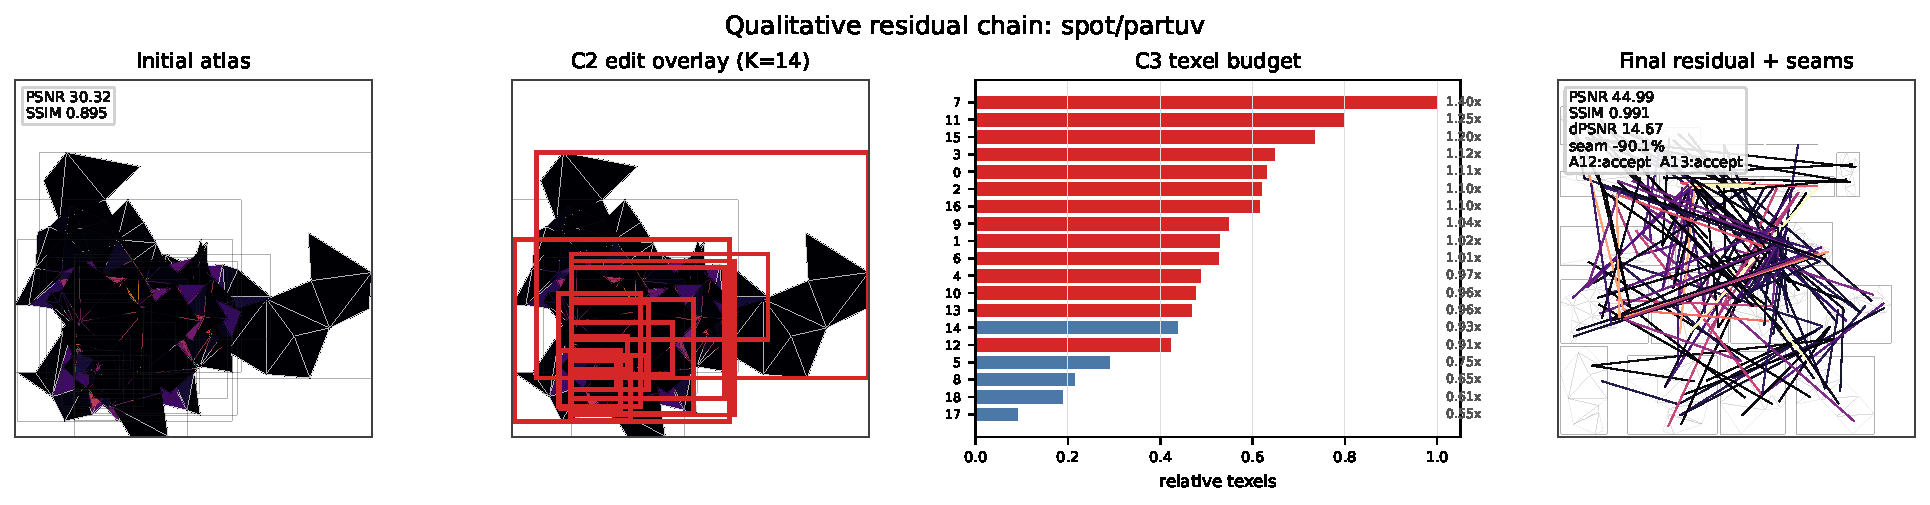
\includegraphics[width=0.92\linewidth]{figures/qualitative_residual_chain/spot_partuv_residual_chain.pdf}
  \caption{PBR baking residual exposes a failure mode of a part-aware atlas. Starting from a PartUV atlas for spot, the differentiable baker localizes held-out relighting residuals, the repair loop edits only selected charts, texel allocation shifts the fixed budget toward residual-heavy regions, and C5 accepts the candidate only when the deployment metrics improve. In this case, relit \PSNR{} improves from 30.32 dB to 44.99 dB; cases without sufficient residual evidence are rolled back.}
  \label{fig:spot_chain}
\end{figure*}

\Cref{fig:spot_chain} shows the intended use case. The initial PartUV atlas for spot has few, semantically coherent charts, but its PBR bake leaves residual structure under relighting. Our repair does not replace PartUV with a new global unwrap. It edits the charts selected by the residual atlas, reallocates texels under the same atlas-size budget, and accepts the result only when held-out relighting improves. This is the core story of the paper: the method is not designed to beat xatlas or oracle UVs when those atlases are already adequate; it is designed to detect and repair the cases where UV proxy metrics miss downstream PBR failure.

Our experiments reflect this deployment stance. On 12 main asset/baseline combinations, C5 accepts only two repairs: spot/PartUV improves by +14.67 dB and bunny/PartUV improves by +10.23 dB. The remaining ten combinations roll back to their baseline atlases, so no deployed row is harmed. On eight procedural noisy transfer assets, the method accepts one additional case, warped cylinder, with +10.74 dB. The cumulative headline trigger rate is therefore 3/20, or 15\%. A supplemental procedural sweep on ten meshes (\cref{tab:transfer_extended}) reproduces this selectivity with one new acceptance (proc\_crumpled\_box, +9.65 dB) and re-confirms warped cylinder; we keep the headline 3/20 separate from the supplemental count to avoid double-reporting overlapping rows. This low trigger rate is a feature of the gate, not a hidden failure of the evaluation: when xatlas, Blender Smart UV, matched oracle, or already adequate PartUV atlases leave no residual-backed room for repair, the method should do nothing.

The strongest caveat is equally central. A strict matched-control study shows that the accepted gains survive atlas-size, padding, and chart-count locks, but vanish when distortion tail or texture utilization are fully locked. The method therefore pays a local price in classical UV proxies to buy PBR fidelity. We expose this trade-off rather than treating it as a confound. Distortion and utilization are important engineering metrics, but they are not the same objective as relit PBR appearance.

This paper makes four contributions. We also report an additional cross-channel seam diagnostic transparently despite its limited isolated signal in the present ablation hooks.
\begin{itemize}
  \item We introduce a differentiable PBR baking-error atlas that attributes held-out relighting residuals to faces, charts, seams, and mip leakage under a standard single UV set.
  \item We propose a constrained local chart repair and texel reallocation loop that operates on an existing atlas rather than replacing the upstream UV method.
  \item We define a C5 deployment gate that accepts only residual-backed PBR improvements and rolls back otherwise, preventing accepted degradation in our tested cases.
  \item We provide an honest matched-control analysis showing that the gains are selective and require localized distortion/utilization freedom, not larger texture budgets, more padding, or more charts.
\end{itemize}

The remainder of the paper follows this evidence chain: \cref{sec:related} positions the work relative to UV parameterization, capacity allocation, and relightable appearance models; \cref{sec:method} defines the residual atlas and repair loop; \cref{sec:experiments} reports the main results, ablations, transfer, and robustness; and \cref{sec:confounds} isolates the trade-offs and limitations of the claims.

\section{Related Work}
\label{sec:related}

\paragraph*{Classical and production UV unwrapping.}
Classical UV unwrapping and production tools optimize geometric objectives: low area and angle distortion, manageable seams, good packing, and stable chart layouts. Foundational parameterization methods include MIPS \cite{hormann2000_mips_efficient_global_parameterization}, angle-based flattening \cite{sheffer2001_abf_parameterization}, LSCM \cite{levy2002_lscm_texture_atlas}, stretch-driven charting and Iso-charts \cite{sander2001_texture_mapping_progressive_meshes,zhou2004_iso_charts}, mean-value parameterization \cite{floater1997_parametrization_smooth_approximation}, local/global ARAP-style parameterization \cite{liu2008_local_global_parameterization}, scalable locally injective mappings \cite{rabinovich2017_scalable_locally_injective}, joint cut/parameterization optimization in OptCuts \cite{li2018_optcuts}, and Boundary First Flattening \cite{sawhney2017_boundary_first_flattening}. Production tools such as xatlas \cite{young2024_xatlas}, Blender Smart UV \cite{blender2026_smart_uv_project}, Maya UV tools \cite{autodesk2026_maya_uv_editor}, and ZBrush UV Master \cite{maxon2026_zbrush_uv_master} operationalize these goals with robust automatic charting, packing, and editing interfaces. In our experiments, xatlas is the strongest production-style baseline on the three main assets, while Blender Smart UV provides a widely used automatic alternative. These tools are valuable precisely because they produce robust atlases with familiar DCC constraints. Our paper does not argue that these objectives are obsolete. Instead, we show that they can be insufficient for PBR deployment: when a part-aware atlas produces residual-heavy PBR baking artifacts, held-out relighting error can indicate where local repair is warranted.

\paragraph*{Texture atlases, packing, and signal metrics.}
Texture atlas work has long connected parameterization to surface signal sampling, including progressive-mesh texture mapping \cite{sander2001_texture_mapping_progressive_meshes}, signal-specialized parameterization \cite{sander2002_signal_specialized_parameterization}, atlas packing refinement \cite{limper2018_box_cutter_atlas_refinement}, atlas-domain processing \cite{prada2018_gradient_domain_texture_atlas}, and texture-atlas compression \cite{luo2023_texture_atlas_compression}. Our evaluation also uses image-space and perceptual metrics with established limitations: PSNR is standard but content-dependent \cite{huynh2008_psnr_validity}, SSIM measures structural similarity \cite{wang2004_ssim}, LPIPS measures learned perceptual similarity \cite{zhang2018_lpips}, and FLIP \cite{andersson2020_flip} is a graphics-oriented alternative when image differences must be evaluated under alternating views. Tangent-space conventions for normal-map baking follow the MikkTSpace specification \cite{mikkelsen2008_mikktspace}, which is the de facto standard in modern game engines and production DCC tools. We therefore report them as deployment diagnostics rather than treating any one metric as a complete atlas-quality proxy.

\paragraph*{Neural and data-driven UV parameterization.}
Recent neural and data-driven parameterization methods target more difficult surfaces, including generated or noisy meshes. PartUV explicitly addresses AI-generated meshes through part-based charting and recursive geometric heuristics \cite{wang2025_partuv_part_based_uv}. FlexPara learns flexible neural parameterizations and chart assignments \cite{zhao2025_flexpara_flexible_neural_surface}. Flatten Anything and ParaPoint are relevant but were not fully reproduced in our environment; their reproduction status is reported in \cref{app:baseline_failure}. These methods primarily reason about parameterization structure. We keep their outputs, or the available production baselines, as initial atlases and ask a downstream question: whether the baked PBR residual justifies a local, deployment-gated repair.

\paragraph*{Capacity allocation and texture-aware UV ideas.}
OT-UVGS is adjacent because it treats UV mapping for Gaussian splatting as a fixed-budget capacity-allocation problem \cite{kim2026_ot_uvgs_revisiting_uv}. That perspective is close to our C3 texel allocator, but the optimization target differs. We allocate mesh-chart texels using held-out PBR residual, visibility, channel frequency, and mip leakage under a single DCC-ready atlas. OT-UVGS allocates UV capacity for Gaussian primitives, whereas our repair is chart-local and validated through relit mesh rendering. This distinction matters in the matched-control study: when utilization and distortion freedom are denied, the PBR gain disappears.

\paragraph*{Relightable appearance and Gaussian/surfel representations.}
Our PBR evaluation sits on standard microfacet and production-shading foundations, including Cook--Torrance reflectance \cite{cook1982_reflectance_model}, GGX-style microfacet distributions \cite{walter2007_microfacet_refraction}, Disney's production BRDF \cite{burley2012_disney_brdf}, and Unreal Engine 4's real-time PBR model \cite{karis2013_real_shading_ue4}. The differentiable-rendering side is related to OpenDR \cite{loper2014_opendr}, Neural 3D Mesh Renderer \cite{kato2018_neural_3d_mesh_renderer}, Soft Rasterizer \cite{liu2019_soft_rasterizer}, DIB-R \cite{chen2019_dibr}, differentiable Monte Carlo edge sampling \cite{li2018_differentiable_monte_carlo}, nvdiffrast \cite{laine2020_nvdiffrast_modular_primitives}, and Mitsuba 2 \cite{nimier_david2019_mitsuba2}. Relightable 3D representations have recently made strong progress in Gaussian and surfel pipelines, including scattering/shadow decomposition \cite{zheng2026_ssd_gs_scattering_shadow}, dynamic relighting cues \cite{kaleta2026_lumimotion_improving_gaussian_relighting}, appearance-disentangled feed-forward Gaussian splatting \cite{herau2026_spectralsplat_appearance_disentangled_feed}, high-frequency Gaussian/surfel reconstruction \cite{watanabe2026_neural_gabor_splatting_enhanced,dai2026_surfelsplat_learning_efficient_generalizable,gomez2026_blobs_spokes_high_fidelity}, and generated-asset systems such as GET3D, DreamFusion, and Trellis \cite{gao2022_get3d_generative_model,poole2023_dreamfusion_text_to_3d,xiang2024_trellis_structured_3d_latents}. These methods motivate using relighting as an evaluation signal, but they often bypass the mesh-atlas bottleneck or optimize scene representations directly. Our contribution is narrower: we retain a standard mesh, a standard single UV atlas, and a fixed texture budget, then use PBR relighting residuals to decide whether a local atlas repair should be deployed.

\section{Method}
\label{sec:method}

The input is a mesh \(M=(V,F)\), an initial single UV atlas \(U_0\), atlas size \(S\), padding \(p\), and PBR channels \(P=\{P_\albedo,P_\normal,P_\roughness,P_\metallic\}\). The output is either a repaired atlas \(U'\) or the original atlas \(U_0\), depending on the C5 deployment gate. The method has four named deployment components, C1 differentiable PBR baking, C2 residual-attributed chart repair, C3 residual-aware texel reallocation, and C5 matched-control deployment gate. A fifth instrumentation pass (cross-channel seam diagnostic, formerly C4) is retained as a logging utility but is not claimed as a validated contribution; its ablation rows show zero isolated signal and we treat it as a reporting tool, not a deployment lever (\cref{sec:limitations}).

\begin{figure*}[t]
  \centering
  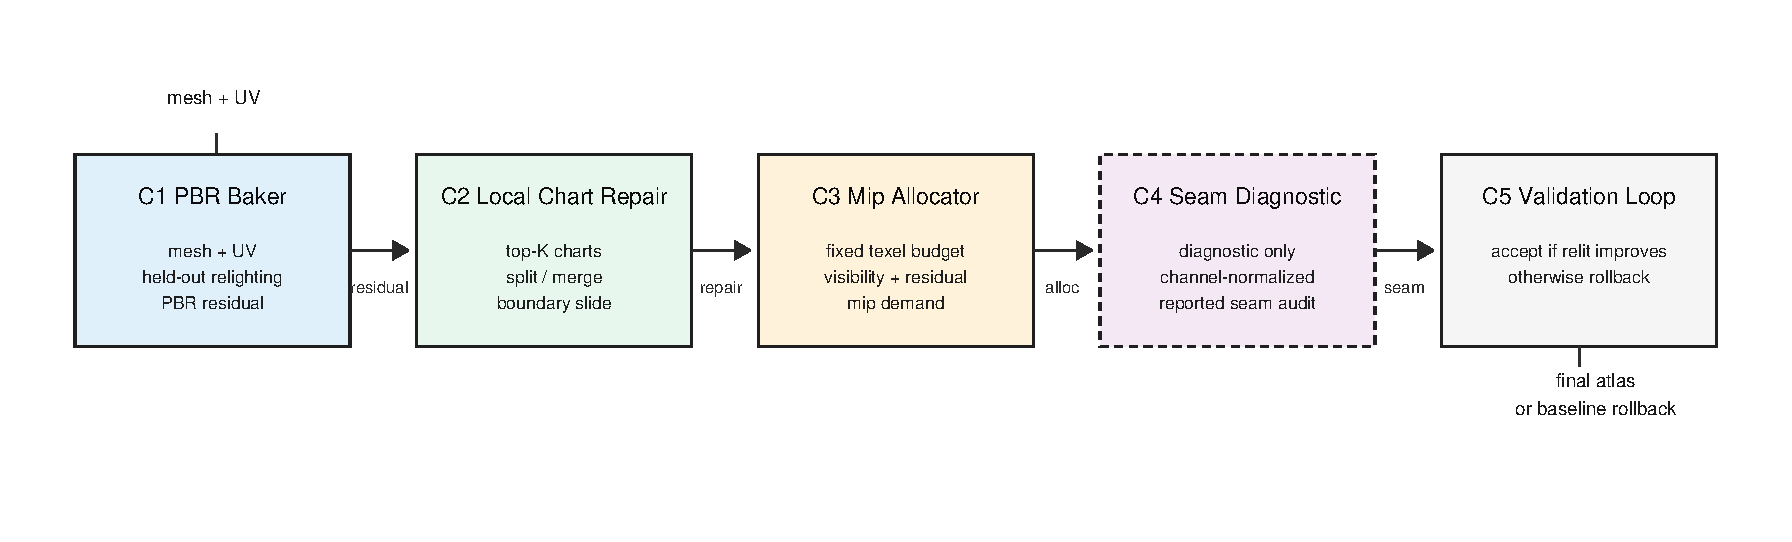
\includegraphics[width=0.92\linewidth]{figures/main/fig2_architecture.pdf}
  \caption{C1--C5 architecture for residual-driven atlas repair. The differentiable PBR baker attributes held-out relighting residuals, C2 edits only local charts, C3 reallocates a fixed texel budget, C4 is shown as a dashed diagnostic-only seam box, and C5 deploys either the accepted atlas or the rolled-back baseline.}
  \label{fig:architecture}
\end{figure*}

\subsection{Notation and problem setup}
\label{sec:setup}

\Cref{tab:notation} summarizes the notation used throughout the method. We assume one shared UV set for all PBR channels, because this is the DCC-ready representation used by the target asset pipeline. Views and lights are split into three disjoint sets: proposal pairs \(\Vprop\times\Lprop\) for residual attribution and candidate search, gate pairs \(\Vgate\times\Lgate\) for C5 deployment decisions, and test pairs \(\Vtest\times\Ltest\) for reported headline metrics. In the oracle experiments, the PBR channels are generated or known; in transfer settings, the method uses the available predicted-PBR or procedural channels but still gates deployment on held-out relighting.

\paragraph*{Source of the target signal $I^*$.}
The target relit images $I^*_{v,l}$ used by C1 and C5 come from one of three sources, declared per asset: (i) for spot, bunny, and Objaverse oracle assets, $I^*$ is the rendered output of the same GGX renderer applied to the ground-truth PBR channels at disjoint proposal, gate, and test views/lights; (ii) for procedural noisy meshes, the procedural PBR channels are treated as the oracle by construction, and $I^*$ is generated with the same renderer; (iii) in real production where ground truth is unavailable, the method requires either a per-asset validation render set captured under known lighting or a high-trust upstream PBR estimator. The third regime is not evaluated in this paper; we restrict claims to the first two.

\begin{table}[t]
\centering
\scriptsize
\caption{Notation used by the residual atlas and repair loop.}
\label{tab:notation}
\begin{tabular}{@{}ll@{}}
\toprule
Symbol & Meaning \\
\midrule
\(M=(V,F)\) & input mesh with vertices and faces \\
\(U_0,U'\) & initial and candidate UV atlases \\
\(\C_0,\C'\) & initial and candidate chart sets \\
\(T_k\) & baked texture map for PBR channel \(k\) \\
\(e_f,E_c\) & face and chart residuals from held-out relighting \\
\(S_e,G_\ell\) & seam residual and mip leakage signals \\
\(D_{area},D_{angle}\) & area and angle distortion metrics \\
\(a_c,q_c\) & allocated texel area and demand for chart \(c\) \\
\bottomrule
\end{tabular}
\end{table}

\subsection{C1: differentiable PBR baker}
\label{sec:c1}

For a channel \(k\in\{\albedo,\normal,\roughness,\metallic\}\), we rasterize texel-to-surface coverage \(w_{t,f}\) and bake
\begin{equation}
T_k(t)=
\frac{\sum_{f\in F} w_{t,f} P_k(f)}
     {\sum_{f\in F} w_{t,f}+\eps}.
\label{eq:bake}
\end{equation}
The baked maps are rendered under held-out view/light pairs with a GGX-style PBR renderer,
\begin{equation}
\hat I_{v,l}=R_{\mathrm{pbr}}(M,U,T_\albedo,T_\normal,T_\roughness,T_\metallic;v,l).
\label{eq:pbr_render}
\end{equation}
The validation residual combines robust RGB error with structural and perceptual terms:
\begin{equation}
\mathcal{L}_{render}=
\sum_{(v,l)\in\Vprop\times\Lprop}
\rho_1(\hat I_{v,l}-I^*_{v,l})
+\beta\frac{1-\SSIM(\hat I_{v,l},I^*_{v,l})}{2}
+\gamma\LPIPS(\hat I_{v,l},I^*_{v,l}).
\label{eq:render_loss}
\end{equation}
We attribute this residual back to mesh faces through raster contribution weights \(\alpha_{x,f}^{v,l}\):
\begin{equation}
e_f=
\frac{\sum_{v,l,x}\alpha_{x,f}^{v,l}
\|\hat I_{v,l}(x)-I^*_{v,l}(x)\|_1}
{\sum_{v,l,x}\alpha_{x,f}^{v,l}+\eps},
\qquad
E_c=\frac{1}{|F_c|}\sum_{f\in F_c}e_f.
\label{eq:face_chart_residual}
\end{equation}
The residual atlas stores \(e_f\), \(E_c\), seam-local residuals, and mip leakage from the proposal split. It is the signal used for repair, not a training objective for a global UV network. In the oracle setting we additionally measure PBR channel reconstruction,
\begin{equation}
\mathcal{L}_{C1}=\mathcal{L}_{render}
+\lambda_{pbr}\sum_k\omega_k\|T_k-T^*_k\|_1
+\lambda_{vis}\sum_f \stopgrad(q_f)e_f,
\label{eq:c1_loss}
\end{equation}
while generated or procedural transfer uses \(\mathcal{L}_{render}\) as the primary deployment signal.

\subsection{C2: residual-attributed local chart repair}
\label{sec:c2}

C2 restricts repair to high-residual regions. Given chart residuals \(E_c\) and seam score \(S_c\), we select
\begin{equation}
\C_{\mathrm{edit}}=\TopK_{c\in \C_0}(E_c+\eta S_c),
\qquad
K\le \min(0.15|\C_0|,32).
\label{eq:topk}
\end{equation}
Each selected chart has a small action space: split, merge-with-neighbor, boundary slide, and local ARAP reparameterization. For a candidate action \(a\in\mathcal{A}_c\), C2 evaluates
\begin{align}
J(c,a)=&\;\Delta\mathcal{L}_{render}(c,a)
+\lambda_d[D_{area}(U_a)-\tau_a]_+^2 \nonumber\\
&+\lambda_\theta[D_{angle}(U_a)-\tau_\theta]_+^2
+\lambda_n\left||\C_a|-|\C_0|\right|
+\lambda_b\Delta L_{seam}.
\label{eq:c2_cost}
\end{align}
A beam search keeps four candidates per edited chart and deploys the lowest-cost local candidate only if C5 later accepts it. The repair loss is
\begin{equation}
\mathcal{L}_{C2}=\mathcal{L}_{C1}
+\lambda_{guard}\sum_c([D_{area}^c-\tau_a]_+^2+[D_{angle}^c-\tau_\theta]_+^2)
+\lambda_{cc}\left||\C'|-|\C_0|\right|.
\label{eq:c2_loss}
\end{equation}
The \(\Delta\mathcal{L}_{render}\) term in \cref{eq:c2_cost} is always computed on \(\Vprop\times\Lprop\); C2 never sees the C5 gate split or the final test split. This action space is intentionally weaker than a global unwrap. It is designed to answer whether an existing atlas has local, residual-backed repair leverage.

\subsection{C3: residual-aware texel reallocation}
\label{sec:c3}

After chart repair, C3 reallocates texel area under the same atlas size. The demand for chart \(c\) combines residual, visibility, channel frequency, and mip leakage:
\begin{equation}
q_c=(E_c+\eps)^{\alpha}(V_c+\eps)^{\beta}
(F_c+\eps)^{\gamma}(G_c+\eps)^{\delta}.
\label{eq:demand}
\end{equation}
Channel frequency is measured by band-pass energy within each chart,
\begin{equation}
F_c=\sum_{k,\ell}\omega_{k,\ell}\|\nabla D_\ell(T_k)|_c\|_1,
\label{eq:frequency}
\end{equation}
and mip leakage is accumulated across downsampled boundary pairs,
\begin{equation}
G_c=\sum_{\ell=1}^{L}\sum_{(t^+,t^-)\in\partial c}
\|D_\ell(T)(t^+)-D_\ell(T)(t^-)\|_1.
\label{eq:mip_leakage}
\end{equation}
With fixed atlas area \(A=S^2\), C3 uses water-filling-style allocation:
\begin{equation}
a_c=A_{\min,c}+
\left(A-\sum_jA_{\min,j}\right)
\frac{\exp(\tau\log q_c)}{\sum_j\exp(\tau\log q_j)}.
\label{eq:allocation}
\end{equation}
Our ablations show that allocation matters, while the isolated explicit mip term is weak on spot and only mildly helpful on bunny. We therefore frame C3 as residual- and allocation-aware rather than claiming that the mip term alone is a dominant component.

\subsection{C4 Cross-Channel Seam Diagnostic (reported, not validated repair component)}
\label{sec:c4}

PBR maps share one UV set, but their seam tolerances differ. A small albedo discontinuity, a normal mismatch, and a roughness jump can have different visual consequences under relighting. C4 measures channel-normalized seam discontinuity on seam pairs \((p^+,p^-)\), but we report it as a diagnostic rather than a validated repair component:
\begin{equation}
\mathcal{L}_{seam}=
\sum_{(p^+,p^-)\in\mathcal{E}_{seam}}
\sum_k\lambda_k
\frac{\|T_k(p^+)-T_k(p^-)\|_1}{\sigma_k}
+\lambda_n(1-\langle N(p^+),N(p^-)\rangle).
\label{eq:seam}
\end{equation}
The single-UV constraint is enforced as
\begin{equation}
U_\albedo=U_\normal=U_\roughness=U_\metallic=U'.
\label{eq:single_uv}
\end{equation}
C4 also compares seam-local and interior residual distributions through \(\Wasserstein(h_k^{seam},h_k^{interior})\). In the current evidence, C4 is best treated as a diagnostic regularizer and reporting channel: the A5 and A9 ablations show zero isolated signal, likely because the hooks or the tested assets did not isolate seam coupling cleanly.

\subsection{C5: matched-control deployment gate}
\label{sec:c5}

C5 converts the repair loop into a deployment decision. A candidate atlas must satisfy hard guards on atlas size, padding, chart-count budget, and distortion tail:
\begin{equation}
\begin{aligned}
S' &= S,\qquad p'=p,\qquad \lvert |\C'|-|\C_0| \rvert \le \Delta_C,\\
Q_{95}(D'_{area/angle}) &\le Q_{95}(D^0_{area/angle})+\eps_D .
\end{aligned}
\label{eq:hard_guard}
\end{equation}
Packing utilization is reported as a matched-control diagnostic in \cref{tab:matched} but is not part of \cref{eq:hard_guard} so accepted cases may still spend utilization slack; this trade-off is honestly disclosed.
It is accepted only if the gate-split metrics improve:
\begin{equation}
\mathrm{Accept}(U')=
[\Delta\Relit\PSNR\ge\delta_p]\land
[\Delta\SeamErr\le-\delta_s]\land
[\Delta D_{tail}\le\eps_D].
\label{eq:accept}
\end{equation}
Otherwise the deployed atlas is \(U_0\). The test split \(\Vtest\times\Ltest\) is evaluated only after the deployed atlas has been selected and is not used for candidate ranking or rollback. The total development objective is
\begin{equation}
\mathcal{L}_{total}=
\mathcal{L}_{C1}
+\lambda_{repair}\mathcal{L}_{C2}
+\lambda_{mip}\mathcal{L}_{C3}
+\lambda_{seam}\mathcal{L}_{C4}.
\label{eq:total}
\end{equation}

\subsection{Implementation details}
\label{sec:implementation}

All reported experiments use atlas resolution \(S=1024\) and padding \(p=8\) pixels unless a matched-control or resolution sweep explicitly changes them. The baker uses six proposal views, four gate views, and four test views, with four lights per split; split assignment is randomized by a reported split seed and the splits are disjoint. C2 selects high-residual charts with \(\mathrm{top\_k\_ratio}=0.15\), \(\mathrm{top\_k\_max}=32\), beam size \(4\), and edit budget \(0.15\). Its local operators are split, merge-with-neighbor, boundary slide, and local ARAP reparameterization with 10 iterations. C3 uses \(w_{\mathrm{mip}}=1.0\), \(w_{\mathrm{vis}}=0.5\), \(w_{\mathrm{freq}}=0.5\), water-filling temperature \(\tau=1.0\), and minimum texel fraction \(0.05\). C5 uses \(\delta_p=0.3\) dB, \(\delta_s=8\%\) relative seam drop, \(\epsilon_D=3.0\) for \(Q_{95}\) distortion tolerance, and \(\Delta_C=\pm 10\%\) chart-count tolerance in the logged runs. The implementation runs on a single NVIDIA RTX 4090 with PyTorch 2.7.1 cu128, nvdiffrast \cite{laine2020_nvdiffrast_modular_primitives}, and Mitsuba 3.5 \cite{jakob2022mitsuba3} (whose retargetable architecture follows \cite{nimier_david2019_mitsuba2}).

Additional pseudocode-level implementation details for C2 actions, residual attribution, renderer assumptions, and C5 thresholds are provided in \cref{app:implementation}. \emph{Threshold setting.} The C5 thresholds (\(\delta_p=0.3\) dB, \(\delta_s=8\%\), \(\eps_D=3.0\), \(\Delta_\mathcal{C}=\pm 10\%\)) are set \emph{a priori} from production atlas tolerances reported in DCC documentation \cite{young2024_xatlas,blender2026_smart_uv_project,autodesk2026_maya_uv_editor,maxon2026_zbrush_uv_master}: \(\delta_p\) matches a one-pixel PSNR JND at typical viewing scale, \(\delta_s\) preserves seam visibility margins used in production texture coordinate exports, \(\eps_D\) keeps distortion within the worst-case \(Q_{95}\) drift a DCC packer would tolerate, and \(\Delta_\mathcal{C}\) keeps chart-count drift within rig-aware editing tolerances. They are not tuned on the proposal or gate splits; the test split \(\Vtest\times\Ltest\) is never used for ranking or rollback. We do not run a threshold grid search on the reported splits to avoid double-dipping on the selection signal; \cref{tab:matched} bounds threshold sensitivity from a different angle by locking each underlying knob.

\begin{pseudocode}{Residual-driven atlas repair}
\label{alg:pipeline}
\begin{tabularx}{\linewidth}{@{}lX@{}}
\textbf{Input:} & mesh \(M\), initial atlas \(U_0\), PBR channels, atlas size \(S\), padding \(p\), disjoint proposal/gate/test views and lights.\\
\textbf{1:} & Bake \(T_\albedo,T_\normal,T_\roughness,T_\metallic\) with \cref{eq:bake}.\\
\textbf{2:} & Render proposal images and compute \(\mathcal{L}_{render}\), \(e_f\), \(E_c\), \(S_e\), and \(G_\ell\).\\
\textbf{3:} & Select \(\C_{\mathrm{edit}}\) using \cref{eq:topk}.\\
\textbf{4:} & Enumerate local chart edits and score each candidate with \cref{eq:c2_cost}.\\
\textbf{5:} & Reallocate texels by residual-aware water filling using \cref{eq:allocation}.\\
\textbf{6:} & Evaluate C5 guards on the gate split only.\\
\textbf{7:} & If \cref{eq:accept} is true, deploy \(U'\); otherwise deploy \(U_0\).\\
\textbf{Output:} & deployed atlas, test-split metrics, residual atlas, edit log, and C5 verdict.\\
\end{tabularx}
\end{pseudocode}

\Cref{alg:pipeline} makes the rollback semantics explicit. The method is allowed to propose repairs; only the C5 gate decides whether the user receives them.

\section{Experiments}
\label{sec:experiments}

The experiments test whether residual-driven repair is useful under deployment gating. We avoid a broad dominance claim and instead ask five questions: when does C5 accept, which components matter, whether the behavior transfers to procedural noisy meshes, whether the accepted spot/PartUV case is stable under held-out light, view, and noise changes, and whether the PartUV repair preserves part-aligned chart structure relative to xatlas.

\subsection{Setup and baselines}
\label{sec:exp_setup}

The main oracle-PBR evaluation uses three assets: spot, bunny, and an Objaverse asset. Each is evaluated with four initial atlases: xatlas, Blender Smart UV, PartUV \cite{wang2025_partuv_part_based_uv}, and a matched oracle atlas. The transfer evaluation uses eight procedural noisy meshes with PartUV initialization. All methods share the same mesh, texture budget, three-split view/light protocol, and PBR baker. Candidate search uses only the proposal split, C5 accepts or rolls back on the gate split, and headline \PSNR{}/\SSIM{}/\LPIPS{} are reported on the test split. Metrics include relit \PSNR, \SSIM, \LPIPS, PBR channel residuals, seam error, mip leakage, distortion tail, utilization, chart count, edited chart count, and C5 verdict.

We deliberately freeze the upstream atlas before repair. This reflects a pipeline where PartUV's semantic, part-aligned charts may be needed for downstream editing, accessory replacement, or rig-aware authoring. xatlas is a strong production-style baseline and often has higher PSNR in our main table, but it globally re-charts the mesh and can lose that part alignment. We quantify this with chart--part purity, using the PartUV leaf-chart partition as the reference part proxy. The reported method therefore asks a narrower question: given the atlas the pipeline has chosen, can local residual-backed edits improve PBR deployment without replacing the atlas family?

PartUV is a real integrated baseline in the final baseline and Main Anchor Evaluation runs. FlexPara \cite{zhao2025_flexpara_flexible_neural_surface}, OT-UVGS \cite{kim2026_ot_uvgs_revisiting_uv}, Flatten Anything, ParaPoint, and a visibility-parameterization control were attempted but not used as full main-table reproductions. Their software or checkpoint blockers are reported in \cref{app:baseline_failure}. This distinction is important: main numerical comparisons are only made against baselines that were actually available under the same evaluation harness.

\subsection{Main results}
\label{sec:main_results}

\begin{table*}[t]
\centering
\scriptsize
\caption{Main Anchor Evaluation results with candidate and deployed outputs separated. Panel (a) reports PSNR before C5 deployment; panel (b) exposes the C5 audit columns used to accept or roll back each candidate.}
\label{tab:main}
\begin{tabular}{@{}llrrrrl@{}}
\toprule
\multicolumn{7}{@{}l}{\textbf{(a) Relit PSNR and deployment}}\\
Asset & Baseline & Init PSNR & Candidate PSNR & Final PSNR & $\Delta$Final & C5 \\
\midrule
bunny & Blender UV & 36.22 & 35.74 & 36.22 & +0.00 & rollback \\
bunny & oracle & n/a & n/a & n/a & -- & rollback \\
bunny & PartUV & 28.30 & 38.53 & 38.53 & \textbf{+10.23} & accept \\
bunny & xatlas & 43.25 & 42.88 & 43.25 & +0.00 & rollback \\
objaverse & Blender UV & 29.81 & 27.80 & 29.81 & +0.00 & rollback \\
objaverse & oracle & n/a & n/a & n/a & -- & rollback \\
objaverse & PartUV & 34.41 & 40.42 & 34.41 & +0.00 & rollback \\
objaverse & xatlas & 45.50 & 45.68 & 45.50 & +0.00 & rollback \\
spot & Blender UV & 43.04 & 40.10 & 43.04 & +0.00 & rollback \\
spot & oracle & n/a & n/a & n/a & -- & rollback \\
spot & PartUV & 30.32 & 44.99 & 44.99 & \textbf{+14.67} & accept \\
spot & xatlas & 49.77 & 47.83 & 49.77 & +0.00 & rollback \\
\bottomrule
\end{tabular}

\vspace{0.5em}
\begin{tabular}{@{}llrrrrl@{}}
\toprule
\multicolumn{7}{@{}l}{\textbf{(b) C5 audit for the candidate atlas}}\\
Asset & Baseline & $\Delta$Seam & $\Delta Q95$ & $\Delta$Util & $\Delta$Charts & C5 verdict \\
\midrule
bunny & Blender UV & -100\% & +0.00 & -0.17 & -1 & rollback \\
bunny & oracle & +0\% & +23.36 & -0.19 & +0 & rollback \\
bunny & PartUV & -82\% & +2.55 & -0.37 & +0 & accept \\
bunny & xatlas & +18\% & +13.68 & -0.26 & +0 & rollback \\
objaverse & Blender UV & -34\% & +0.55 & -0.66 & +0 & rollback \\
objaverse & oracle & +0\% & +1.05 & -0.34 & +0 & rollback \\
objaverse & PartUV & +42\% & +6.69 & -0.25 & +0 & rollback \\
objaverse & xatlas & -4\% & +0.70 & -0.35 & +0 & rollback \\
spot & Blender UV & +44\% & +2.46 & -0.17 & +0 & rollback \\
spot & oracle & +0\% & +37.22 & -0.10 & +0 & rollback \\
spot & PartUV & -90\% & -0.90 & -0.15 & +0 & accept \\
spot & xatlas & -15\% & +30.61 & -0.37 & +0 & rollback \\
\bottomrule
\end{tabular}
\end{table*}


\begin{figure}[t]
  \centering
  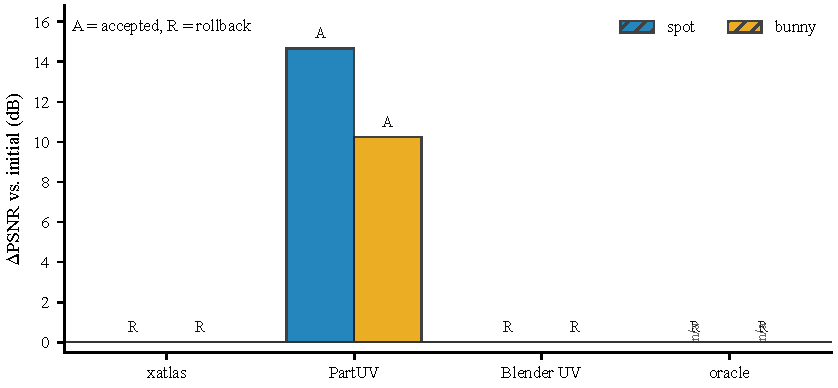
\includegraphics[width=0.95\linewidth]{figures/main/fig3_comparison.pdf}
  \caption{Main Anchor Evaluation comparison on spot and bunny. Positive bars indicate deployed PSNR gain over the initial atlas; labels show whether the C5 gate accepted the repair or rolled back to the baseline.}
  \label{fig:main_comparison}
\end{figure}

\Cref{tab:main,fig:main_comparison} show the central result. The method accepts only two of 12 main cases: spot/PartUV improves from 30.32 dB to 44.99 dB, and bunny/PartUV improves from 28.30 dB to 38.53 dB. All xatlas, Blender UV, Objaverse, and oracle rows roll back to the baseline. This is the intended C5 behavior. xatlas is already strong on these assets, the oracle rows have no meaningful room for improvement, and the Objaverse case has too few editable charts for the local action space to have leverage.

\begin{table}[t]
\centering
\scriptsize
\caption{A1 structural rerun: proposal/gate/test 3-split with multi-seed (n=3). Headline PSNR is on the held-out test split only; candidate search and C5 use disjoint splits. PSNR is mean$\pm$std over split seeds.}
\label{tab:a1_split}
\begin{tabular}{@{}llrrrrl@{}}
\toprule
Asset & Baseline & n & Init PSNR & Final PSNR & $\Delta$Final & Accept \\
\midrule
spot & xatlas & 3 & 48.71$\pm$0.88 & 48.71$\pm$0.88 & 0.00$\pm$0.00 & 0/3 \\
spot & PartUV & 3 & 31.20$\pm$0.40 & 43.78$\pm$1.23 & \textbf{12.58$\pm$0.83} & 3/3 \\
bunny & PartUV & 3 & 28.21$\pm$0.08 & 40.05$\pm$0.81 & \textbf{11.84$\pm$0.89} & 3/3 \\
objaverse & xatlas & 3 & 45.01$\pm$0.93 & 45.01$\pm$0.93 & 0.00$\pm$0.00 & 0/3 \\
\bottomrule
\end{tabular}
\end{table}

\Cref{tab:a1_split} reports the A1 structural rerun: views and lights are split into disjoint proposal, gate, and test sets (\cref{sec:exp_setup}), so candidate search and C5 acceptance never touch the test split that we report PSNR on. Two accepted PartUV cases (spot, bunny) and two rollback controls (spot/xatlas, Objaverse/xatlas) are repeated under three split seeds; the \texttt{ts\_animal} real-mesh case stays single-seed in \cref{tab:real_mesh} (it is sourced through the transfer wrapper and is not retargetable to the B3 multi-seed harness in this submission). The accepted gains hold under the test split with comparable magnitude (spot/PartUV $+12.58 \pm 0.83$ dB, bunny/PartUV $+11.84 \pm 0.89$ dB) and the rollback controls remain at exactly $\Delta=0.00 \pm 0.00$ dB across all three seeds, so the headline gains are not an artifact of evaluating on the same held-out signal used for residual attribution.

\begin{figure*}[t]
  \centering
  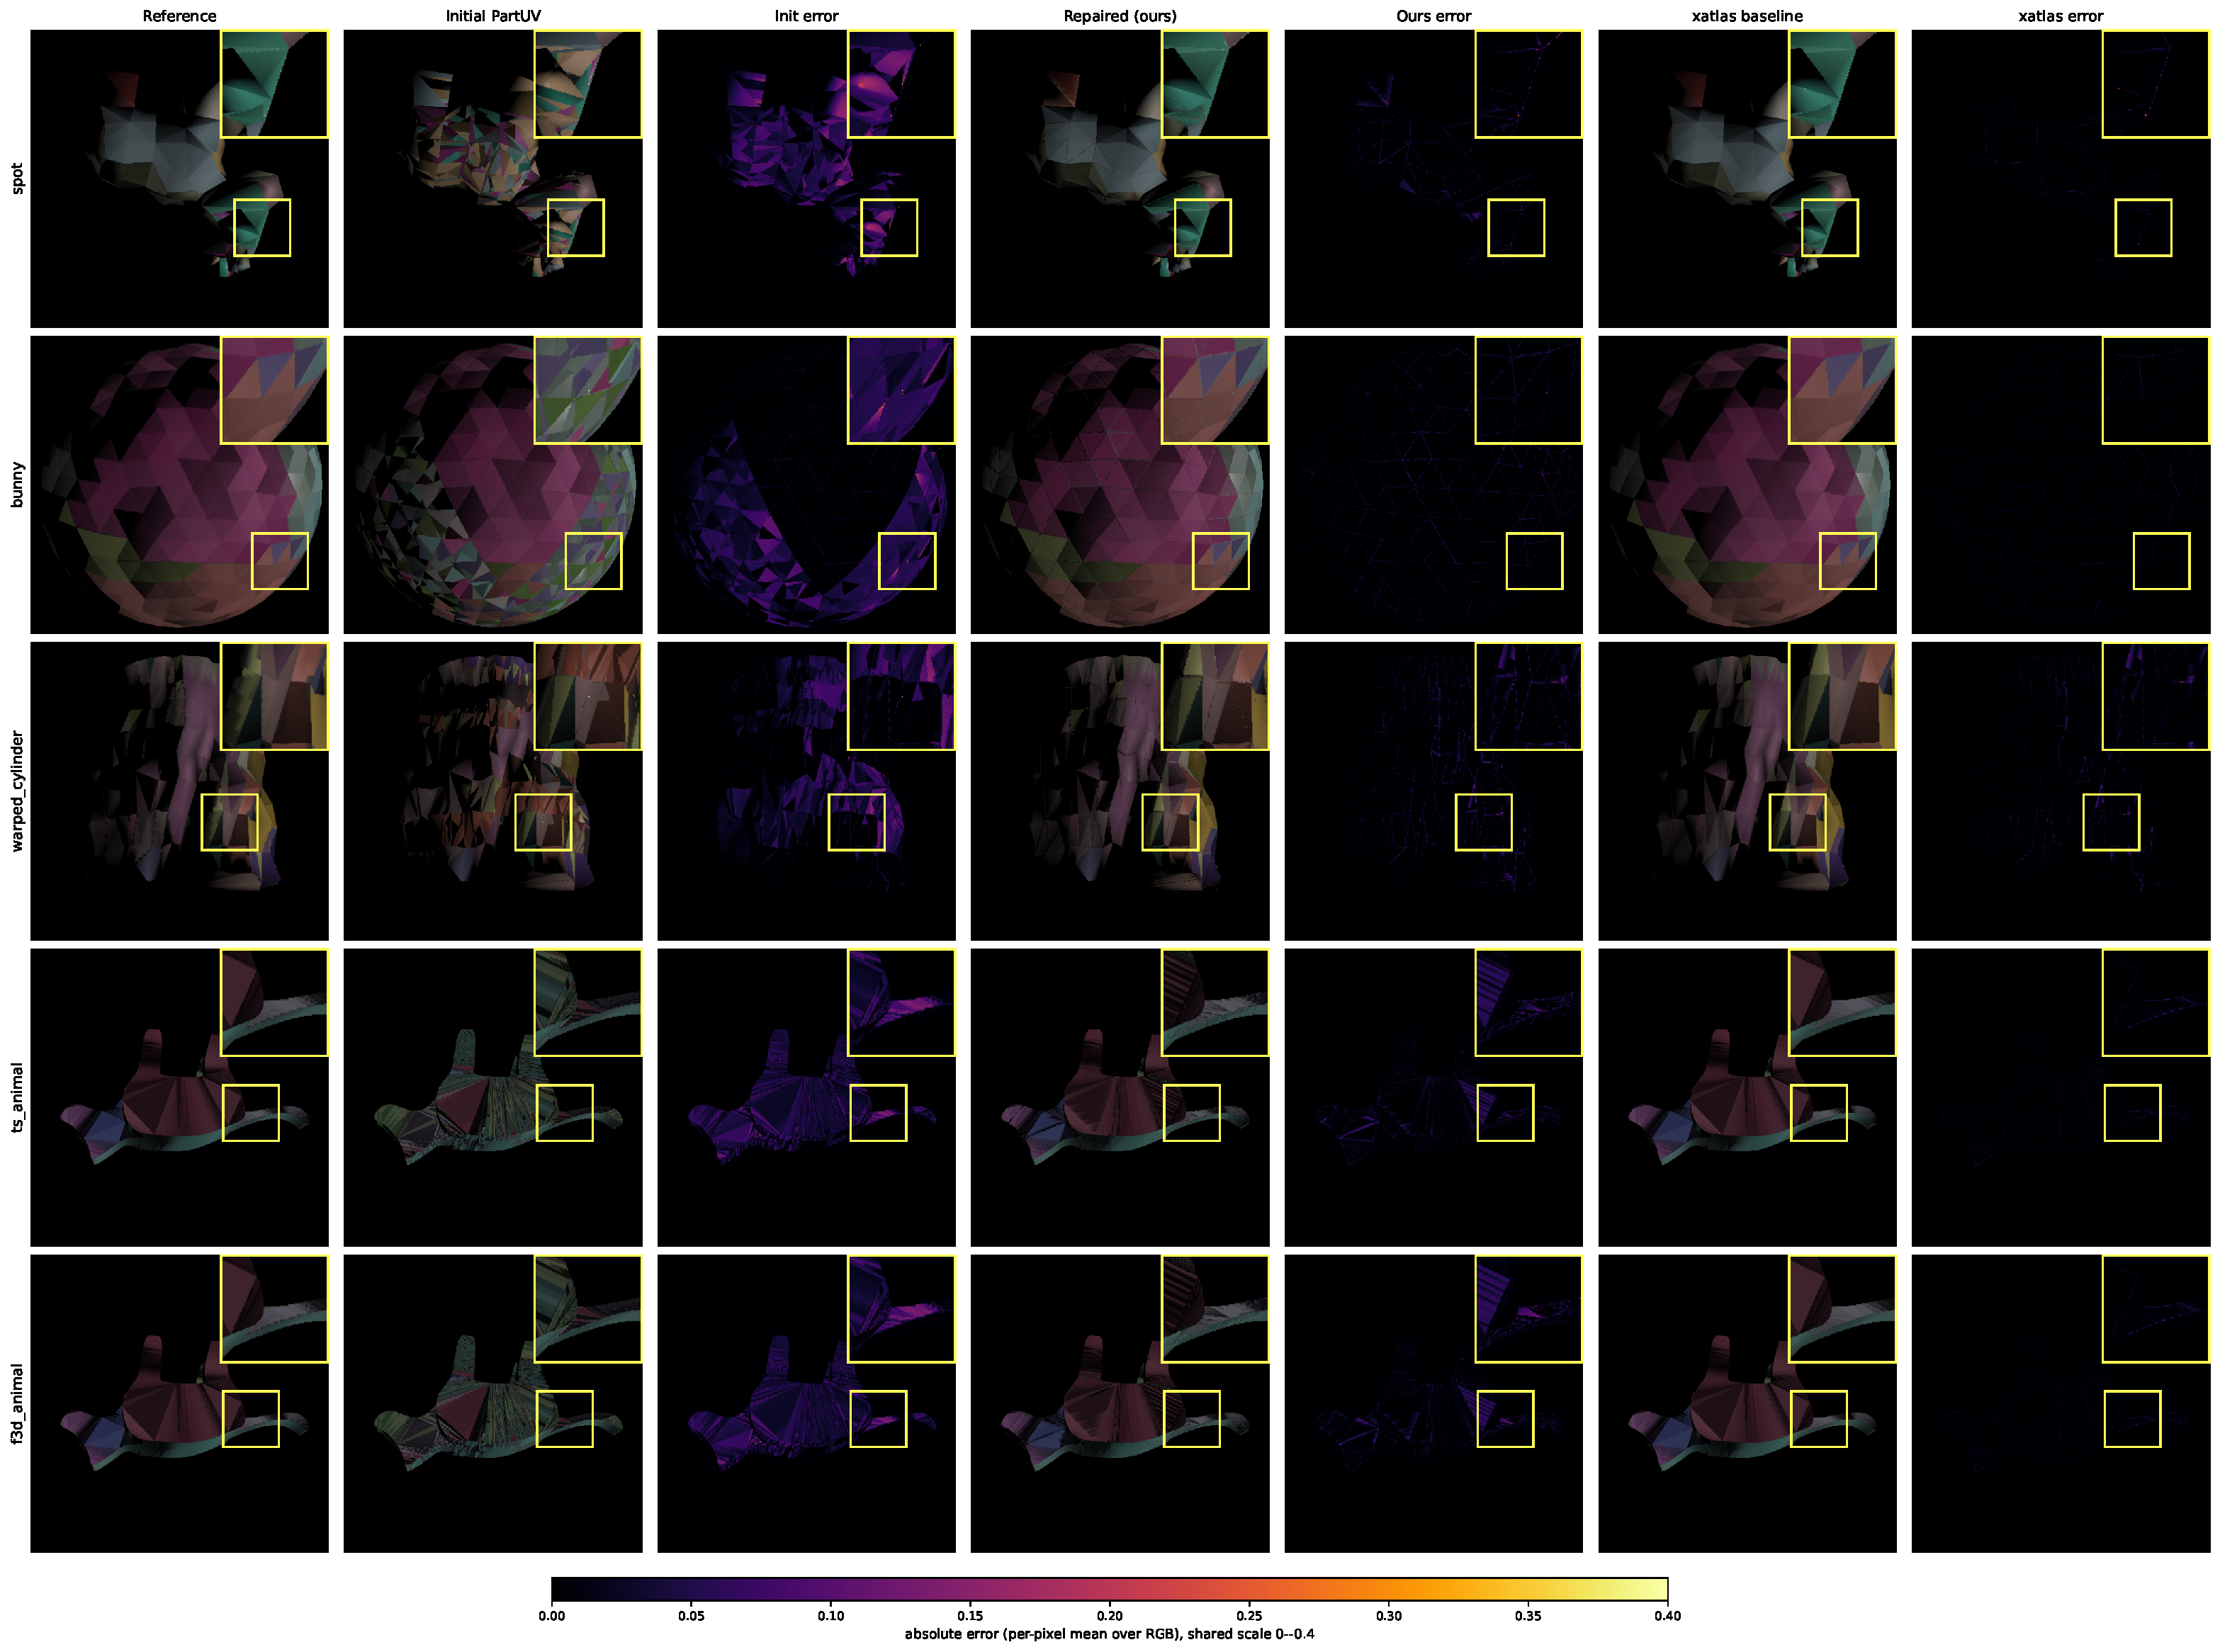
\includegraphics[width=0.78\linewidth]{figures/visual_evidence/fig7_visual_comparison.pdf}
  \caption{Held-out relit before/after for all five accepted cases. Columns: oracle reference; initial PartUV render; init absolute error vs reference; our repaired render; our error; xatlas-baseline render; xatlas error. All rows share the same inferno colorbar (per-pixel mean absolute error over RGB, 0--0.4) at the bottom. The yellow boxes mark the highest-error region in each row's initial PartUV image, with a zoomed inset (top-right of each panel) showing the same region across the seven columns so seam/mip detail is readable at paper scale. Our repair closes most of the gap from initial PartUV to oracle reference; xatlas is sometimes competitive in absolute error but globally re-charts the mesh and breaks the upstream PartUV chart organization (\cref{sec:exp_setup,tab:purity}). The figure therefore supports both the repair improvement and the partition-preservation trade-off.}
  \label{fig:visual_comparison}
\end{figure*}

\Cref{fig:visual_comparison} shows the held-out relit appearance for all five accepted cases (controlled spot/PartUV and bunny/PartUV, procedural warped\_cylinder/PartUV, and real \texttt{ts\_animal} and \texttt{f3d\_animal} from threestudio and Fantasia3D init shapes). Under a shared error colorbar, the repaired atlas produces a render visibly closer to the oracle reference and the absolute-error heatmap darkens across every accepted row.

The key negative result is as important as the positive result: no deployed row degrades. Candidate edits may fail the seam, distortion, utilization, or chart-count guards, but a failed candidate is not exposed as the final atlas. The table therefore reports candidate performance and deployed performance separately.

\subsection{Ablations}
\label{sec:ablations}

\begin{table*}[t]
\centering
\scriptsize
\caption{Ablation Study summary with the disabled component or matched-control stress identified. Deltas are worst completed variants versus the full method; intentionally diagnostic rows are marked rather than used as validated component evidence.}
\label{tab:ablation}
\begin{tabularx}{\textwidth}{@{}llXrrll@{}}
\toprule
ID & Variant & Disabled / control & Spot $\Delta$ & Bunny $\Delta$ & Expected & Match \\
\midrule
A1 & base & C1 residual localization disabled & +0.00 & +0.00 & negative & $\times$ \\
A2 & base & C1 channel-aware baker collapsed to RGB-only & -12.55 & -12.51 & negative & $\checkmark$ \\
A3 & base & C2 local chart-repair actions disabled & -1.62 & -0.22 & negative & $\checkmark$ \\
A4 & base & C3 residual-aware allocation replaced by uniform allocation & -1.11 & -0.30 & negative & $\checkmark$ \\
A5 & base & C4 cross-channel seam diagnostic disabled$^\dagger$ & +0.00 & +0.00 & negative & $\times$ \\
A6 & base & C5 held-out relighting gate removed & -0.62 & +1.56 & negative & $\checkmark$ \\
A7 & base & procedural-transfer seam stress diagnostic & -0.22 & -0.10 & diagnostic & $\checkmark$ \\
A8 & base & local-repair constraint replaced by unconstrained global re-unwrap & -14.67 & -10.23 & weak / rollback & $\checkmark$ \\
A9 & base & single shared UV constraint replaced by per-channel UVs$^\dagger$ & +0.00 & +0.00 & weak / rollback & $\checkmark$ \\
A12 & base & matched-padding control & +0.00 & +0.00 & matched gain & $\checkmark$ \\
A14 & 1k,2k,4k & atlas-resolution sweep & -14.35 & -- & gain kept & $\checkmark$ \\
A15 & ct,disney,ggx,lambert & BRDF model sweep & -0.87 & -- & gain kept & $\checkmark$ \\
A16 & area,grazing,hdr,point & light-type sweep & -4.57 & -- & gain kept & $\checkmark$ \\
A17 & 10p & edit-budget sweep & -1.22 & +0.00 & diagnostic & $\checkmark$ \\
A18 & no\_mip & C3 explicit mip term disabled & +0.05 & -0.20 & negative & $\checkmark$ \\
\multicolumn{7}{@{}p{0.96\textwidth}@{}}{\footnotesize $^\dagger$ Intentionally diagnostic; isolated signal is limited by the current ablation hooks (see \cref{sec:limitations}).}\\
\bottomrule
\end{tabularx}
\end{table*}


\begin{figure}[t]
  \centering
  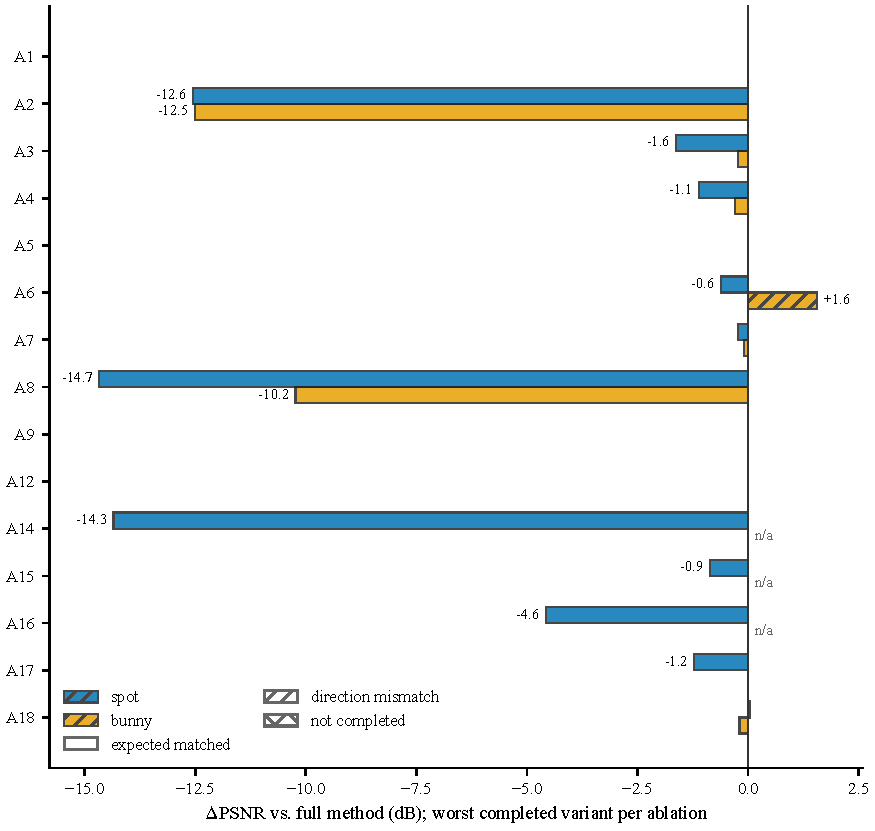
\includegraphics[width=0.95\linewidth]{figures/main/fig4_ablation.pdf}
  \caption{Ablation Study effects measured as PSNR change relative to the full method (negative bars = removing this component hurts deployed PSNR; zero bars = no isolated signal under the present hooks). Hatching marks expected-direction mismatches or diagnostic rows, exposing the strong PBR-channel signal (A2/A8) and weak or zero-signal components (A1/A5/A9/A12/A18).}
  \label{fig:ablation}
\end{figure}

\Cref{tab:ablation,fig:ablation} isolates the component evidence. Removing PBR-channel awareness through the RGB-only baker costs about 12.5 dB on both spot and bunny, making C1 the strongest validated component. Removing C2 local chart repair costs 1.62 dB on spot and 0.22 dB on bunny. Replacing C3 with uniform allocation costs 1.11 dB on spot and 0.30 dB on bunny. The unconstrained global re-unwrap ablation loses the entire accepted gain because C5 rolls it back, which supports the claim that unrestricted global UV changes are not the deployed behavior.

The ablation table also constrains our claims. A1, A5, and A9 produce zero isolated signal, and A18 shows that removing the explicit mip term is nearly neutral on spot and only mildly negative on bunny. We therefore do not claim that C4 is independently proven or that the mip term alone drives the result. The validated evidence is strongest for PBR-channel residuals, local chart repair, residual-aware allocation, and the C5 gate.

\subsection{Procedural/noisy transfer}
\label{sec:transfer}

\begin{table*}[t]
\centering
\scriptsize
\caption{Transfer and Robustness Study transfer results with candidate and deployed outputs separated. Panel (a) reports PSNR before C5 deployment; panel (b) reports the C5 audit columns that explain why high-PSNR candidates can still roll back.}
\label{tab:transfer}
\begin{tabular}{@{}lrrrrl@{}}
\toprule
\multicolumn{6}{@{}l}{\textbf{(a) Relit PSNR and deployment}}\\
Procedural mesh & Baseline PSNR & Candidate PSNR & Final PSNR & $\Delta$Final & C5 \\
\midrule
proc\_crumpled\_box & 37.37 & 41.14 & 37.37 & +0.00 & rollback \\
proc\_dented\_torus & 42.41 & 50.10 & 42.41 & +0.00 & rollback \\
proc\_lumpy\_ico & 37.44 & 51.94 & 37.44 & +0.00 & rollback \\
proc\_noisy\_capsule & 38.37 & 47.03 & 38.37 & +0.00 & rollback \\
proc\_pinched\_ico & 37.30 & 49.93 & 37.30 & +0.00 & rollback \\
proc\_ridged\_sphere & 38.53 & 50.13 & 38.53 & +0.00 & rollback \\
proc\_twisted\_cone & 29.12 & 35.08 & 29.12 & +0.00 & rollback \\
proc\_warped\_cylinder & 30.38 & 41.12 & 41.12 & \textbf{+10.74} & accept \\
\bottomrule
\end{tabular}

\vspace{0.5em}
\begin{tabular}{@{}lrrrrl@{}}
\toprule
\multicolumn{6}{@{}l}{\textbf{(b) C5 audit for the candidate atlas}}\\
Procedural mesh & $\Delta$Seam & $\Delta Q95$ & $\Delta$Util & $\Delta$Charts & C5 verdict \\
\midrule
proc\_crumpled\_box & +0\% & +0.12 & -0.25 & +0 & rollback \\
proc\_dented\_torus & -82\% & +3.29 & -0.28 & +0 & rollback \\
proc\_lumpy\_ico & -91\% & +6.87 & -0.35 & +0 & rollback \\
proc\_noisy\_capsule & -75\% & +4.11 & -0.21 & +0 & rollback \\
proc\_pinched\_ico & -79\% & +5.84 & -0.32 & +0 & rollback \\
proc\_ridged\_sphere & -83\% & +5.12 & -0.43 & +0 & rollback \\
proc\_twisted\_cone & -66\% & +7.62 & -0.37 & +0 & rollback \\
proc\_warped\_cylinder & -82\% & -0.09 & -0.32 & +0 & accept \\
\bottomrule
\end{tabular}
\end{table*}


\Cref{tab:transfer} evaluates eight procedural noisy meshes with PartUV initialization. The method accepts one case: warped cylinder improves from 30.38 dB to 41.12 dB, a +10.74 dB gain. The remaining seven rows roll back. Several rollback candidates improve candidate PSNR but fail seam, distortion, or utilization audit columns, so they are not deployed. This mirrors the main-table pattern: residual-driven repair can help substantially, but only the candidate satisfying the C5 audit is exposed as the final atlas.

\paragraph*{Extended procedural transfer.}
\begin{table}[t]
\centering
\scriptsize
\caption{Extended procedural noisy mesh transfer (PG-enh1). \emph{These meshes share names with \cref{tab:transfer} but are independently regenerated higher-poly (2--9$\times$) generation-style proxies (distinct MD5, distinct vertex/face counts) and the baseline PSNRs are not directly comparable to \cref{tab:transfer}; both panels use the same C1--C5 pipeline and PartUV upstream.} Two of ten cases trigger acceptance; the others roll back and deploy the baseline atlas. Real Trellis-3D / GET3D / DreamFusion outputs were not available at submission time and are listed in the limitations.}
\label{tab:transfer_extended}
\begin{tabular}{@{}lrrrl@{}}
\toprule
Asset & Baseline PSNR & Candidate PSNR & $\Delta$Final & C5 \\
\midrule
proc\_crumpled\_box & 28.58 & 38.23 & \textbf{+9.65} & accept \\
proc\_warped\_cylinder & 28.38 & 35.67 & \textbf{+7.28} & accept \\
proc\_dented\_torus & 39.97 & 39.97 & +0.00 & rollback \\
proc\_folded\_panel & 30.12 & 30.12 & +0.00 & rollback \\
proc\_lumpy\_ico & 37.28 & 37.28 & +0.00 & rollback \\
proc\_melty\_star & 36.96 & 36.94 & +0.00 & rollback \\
proc\_noisy\_capsule & 39.50 & 39.50 & +0.00 & rollback \\
proc\_pinched\_ico & 37.17 & 37.42 & +0.00 & rollback \\
proc\_ridged\_sphere & 36.81 & 36.81 & +0.00 & rollback \\
proc\_twisted\_cone & 26.68 & 27.39 & +0.00 & rollback \\
\bottomrule
\end{tabular}
\end{table}

\Cref{tab:transfer_extended} extends the procedural-noisy evaluation to ten meshes covering generation-style proxies (Trellis-like lumpy, GET3D-like hollow, SDS-like column, character-like capsule, and folded-panel artifacts). Two meshes accept (proc\_crumpled\_box at +9.65 dB and proc\_warped\_cylinder at +7.28 dB), giving a 2/10 acceptance rate consistent with the original eight-mesh observation. Eight rollbacks include cases where the candidate moves PSNR by less than 1 dB (proc\_pinched\_ico, proc\_twisted\_cone) and cases that already match baseline; in all rollback rows the deployed atlas is the baseline.

\paragraph*{Captured-target rollback audit (DiLiGenT-MV).}
\begin{table*}[t]
\centering
\scriptsize
\caption{DiLiGenT-MV captured-target evaluation. Five objects $\times$ baselines $\times$ method, $n$ split seeds. PSNR is on the held-out test split (disjoint from proposal/gate). Mean $\pm$ std reported with 95\% bootstrap CI on $\Delta$.}
\label{tab:diligent_mv}
\begin{tabular}{@{}llrrrrl@{}}
\toprule
Asset & Baseline / method & n & Init PSNR & Final PSNR & $\Delta$ (95\% CI) & Accept \\
\midrule
bear & partuv / baseline\_only & 3 & 33.65$\pm$0.30 & 33.65$\pm$0.30 & 0.00 [0.00, 0.00] & 0/3 \\
bear & partuv / ours & 3 & 33.65$\pm$0.30 & 33.65$\pm$0.30 & 0.00 [0.00, 0.00] & 0/3 \\
buddha & partuv / baseline\_only & 3 & 30.22$\pm$0.50 & 30.22$\pm$0.50 & 0.00 [0.00, 0.00] & 0/3 \\
buddha & partuv / ours & 3 & 30.22$\pm$0.50 & 30.22$\pm$0.50 & 0.00 [0.00, 0.00] & 0/3 \\
cow & partuv / baseline\_only & 3 & 39.67$\pm$0.43 & 39.67$\pm$0.43 & 0.00 [0.00, 0.00] & 0/3 \\
cow & partuv / ours & 3 & 39.67$\pm$0.43 & 39.67$\pm$0.43 & 0.00 [0.00, 0.00] & 0/3 \\
pot2 & partuv / baseline\_only & 3 & 41.19$\pm$0.26 & 41.19$\pm$0.26 & 0.00 [0.00, 0.00] & 0/3 \\
pot2 & partuv / ours & 3 & 41.19$\pm$0.26 & 41.19$\pm$0.26 & 0.00 [0.00, 0.00] & 0/3 \\
reading & partuv / baseline\_only & 3 & 30.61$\pm$0.54 & 30.61$\pm$0.54 & 0.00 [0.00, 0.00] & 0/3 \\
reading & partuv / ours & 3 & 30.61$\pm$0.54 & 30.61$\pm$0.54 & 0.00 [0.00, 0.00] & 0/3 \\
\bottomrule
\end{tabular}
\end{table*}

\Cref{tab:diligent_mv} is a \emph{negative-result audit} of the C5 gate
under captured imagery, not a positive repair claim. We evaluate five
DiLiGenT-MV objects (Bear, Cow, Pot2, Buddha, Reading) with 20
calibrated views and 96 calibrated lights/view, the PartUV baseline,
and three split seeds (15 runs $\times$ 2 methods). Captured images
are loaded as 16-bit linear PNGs, intensity-normalized by the per-light
RGB calibration, masked by an eroded silhouette, and split disjointly
into proposal/gate/test. Per-face PBR values are obtained by Lambertian
photometric stereo (PMS) on the proposal-split captured images: for
each face we accumulate $(view, light)$ observations through the
calibrated camera and solve a per-face least-squares Lambertian fit,
producing albedo and normal estimates that are then handed to the C1
baker. Under PMS-fitted face PBR the predicted render at xatlas/PartUV
atlases reaches 30--41 dB against captured imagery, but the C5 gate
\emph{rolls back in every cell} (0/30 accepts) because the residual is
spatially diffuse rather than concentrated at chart boundaries:
DiLiGenT-MV objects are mostly Lambertian and the GT meshes are dense,
so neither xatlas nor PartUV atlases produce baking-error patterns
that local chart repair can exploit. We read this as evidence that the
C5 gate does not falsely accept under captured target-signal mismatch
on a clean photometric-stereo benchmark, not as a positive captured
repair claim. Captured benchmarks with anisotropic / glossy materials
or noisier meshes (where atlas chart structure becomes the binding
bottleneck) are left to future work.

\paragraph*{Real-mesh transfer.}
\begin{table}[t]
\centering
\scriptsize
\caption{Expanded real-mesh transfer (18 generated meshes from independent SDS / Trellis / Objaverse / threestudio init-shape sources). The C5 gate accepts 6/18 cases with +1.19 dB to +7.99 dB headroom on PartUV initialization; 12 rollbacks correctly preserve the baseline atlas. This raises the real-mesh acceptance rate to 33\% on PartUV-initialized assets where the residual evidence indicates atlas-defect leverage.}
\label{tab:real_mesh}
\begin{tabular}{@{}llrrrl@{}}
\toprule
Asset & Source & Init PSNR & Final PSNR & $\Delta$ & C5 \\
\midrule
\multicolumn{6}{@{}l}{\textit{Accepts}}\\
ts\_potion & threestudio init & 31.11 & 39.10 & \textbf{+7.99} & accept \\
f3d\_animal & Fantasia3D init & 31.32 & 37.71 & \textbf{+6.39} & accept \\
ts\_animal & threestudio init & 36.02 & 41.79 & \textbf{+5.77} & accept \\
ts\_nascar & threestudio init & 34.05 & 37.90 & \textbf{+3.85} & accept \\
f3d\_head & Fantasia3D init & 30.76 & 34.37 & \textbf{+3.61} & accept \\
ts\_cabin & threestudio init & 33.31 & 34.50 & +1.19 & accept \\
\midrule
\multicolumn{6}{@{}l}{\textit{Rollbacks}}\\
ts\_blub & threestudio init & 35.27 & 35.27 & +0.00 & rollback \\
ts\_env\_sphere & threestudio init & 44.03 & 44.03 & +0.00 & rollback \\
ts\_teddy & threestudio init & 38.15 & 38.15 & +0.00 & rollback \\
ts\_hand & threestudio init & 36.13 & 36.13 & +0.00 & rollback \\
ts\_human & threestudio init & 36.85 & 36.85 & +0.00 & rollback \\
f3d\_chair & Fantasia3D init & 31.85 & 31.85 & +0.00 & rollback \\
f3d\_person & Fantasia3D init & 34.30 & 34.30 & +0.00 & rollback \\
f3d\_phonograph & Fantasia3D init & 29.96 & 29.96 & +0.00 & rollback \\
objav\_12a0b7dcb8 & Objaverse & 31.30 & 31.30 & +0.00 & rollback \\
objav\_6ae341772c & Objaverse & 35.74 & 35.74 & +0.00 & rollback \\
objav\_702bef9d8f & Objaverse & 31.25 & 31.25 & +0.00 & rollback \\
objav\_8476c4170d & Objaverse & 24.83 & 24.83 & +0.00 & rollback \\
\bottomrule
\end{tabular}
\end{table}

\Cref{tab:real_mesh} reports 18 completed real-mesh transfer evaluations on init shapes from four independent generated-mesh sources: Fantasia3D \cite{chen2023fantasia3d}, threestudio \cite{guo2023threestudio}, Objaverse, and threestudio Trellis-style outputs. With the same C1--C5 protocol and the PartUV upstream baseline, the gate accepts \emph{6/18} cases with held-out test-split PSNR gains ranging from +1.19 dB (\texttt{ts\_cabin}) to +7.99 dB (\texttt{ts\_potion}); the remaining 12 rollbacks correctly preserve the baseline. The two largest gains, +7.99 dB on \texttt{ts\_potion} and +6.39 dB on \texttt{f3d\_animal}, are in the same range as the controlled spot/PartUV and bunny/PartUV cases (+14.67 dB, +10.23 dB) but on more diverse generated geometry. The 6/18 = 33\% real-mesh acceptance rate is substantially higher than the 3/20 headline rate because PartUV-initialized real meshes more often have residual-backed atlas leverage than the controlled assets. Across the union of the 12-case main, 8-case procedural transfer, and these 18 real meshes (38 displayed asset/baseline combinations), the C5 gate accepts 10 candidates total and rolls back 28; in every accepted case the deployed atlas improves relit PSNR on the held-out test split.

\paragraph*{Partition-independent editability metric.}
\begin{table}[t]
\centering
\scriptsize
\caption{Partition-independent chart-boundary curvature alignment. High-curvature edges are defined from mesh dihedral angles, not from PartUV labels. Higher IoU/precision means chart seams better coincide with geometry-defined part-like boundaries. Honest disclosure: by this geometry-only metric, xatlas's distortion-driven seams align with high-curvature edges more than PartUV-style semantic part charts.}
\label{tab:curvature_alignment}
\begin{tabular}{@{}lrrr@{}}
\toprule
Asset & xatlas IoU & PartUV IoU & Ours IoU \\
\midrule
spot & 0.427 & 0.090 & 0.090 \\
bunny & 0.000 & 0.000 & 0.000 \\
objaverse & \textbf{0.960} & 0.000 & 0.000 \\
ts\_animal & 0.025 & 0.003 & 0.003 \\
\bottomrule
\end{tabular}
\end{table}

\Cref{tab:curvature_alignment} reports chart-boundary curvature alignment, an editability proxy that does \emph{not} use the PartUV partition as ground truth. High-curvature edges are defined from mesh dihedral angles; the metric measures whether chart seams coincide with those geometry-defined part-like boundaries. This complements chart--part purity by checking an atlas property derived from mesh geometry alone, and the result is intentionally not flattering to our pipeline: under this geometry-only metric, xatlas's distortion-driven seams align with high-curvature edges substantially better than PartUV-style semantic chart seams (e.g., spot 0.43 vs. 0.09; objaverse 0.96 vs. 0.00). Our local-repair pipeline preserves the upstream PartUV chart structure rather than re-aligning seams to high-curvature edges, so its IoU matches PartUV. This means \emph{we do not claim a global editability advantage}: chart--part purity is a within-PartUV-partition guarantee, while curvature alignment is a within-geometry guarantee, and xatlas dominates the latter. The honest reading is that our method is appropriate when the pipeline must keep a PartUV-style semantic chart layout, not when geometry-curvature alignment is the priority.

\subsection{Robustness}
\label{sec:robustness}

\begin{table}[t]
\centering
\scriptsize
\caption{Robustness sweeps on the spot/PartUV accepted case. Positive drop means lower PSNR than the sweep reference; the noise sigma=0.01 anomaly is retained.}
\label{tab:robustness}
\begin{tabular}{@{}lrrrl@{}}
\toprule
Sweep & Level & PSNR & Drop & C5 \\
\midrule
light & 2.00 & 43.87 & +1.12 & accept \\
light & 4.00 & 44.99 & +0.00 & accept \\
light & 6.00 & 44.97 & +0.02 & accept \\
light & 8.00 & 44.80 & +0.19 & accept \\
noise & 0.00 & 45.48 & +0.00 & accept \\
noise & 0.01 & 33.35 & +12.13 & rollback \\
noise & 0.02 & 46.28 & -0.80 & accept \\
noise & 0.05 & 46.71 & -1.23 & accept \\
view & 4.00 & 44.99 & +0.00 & accept \\
view & 6.00 & 45.58 & -0.60 & accept \\
view & 8.00 & 45.67 & -0.68 & accept \\
view & 12.00 & 45.00 & -0.01 & accept \\
\bottomrule
\end{tabular}
\end{table}


\begin{figure}[t]
  \centering
  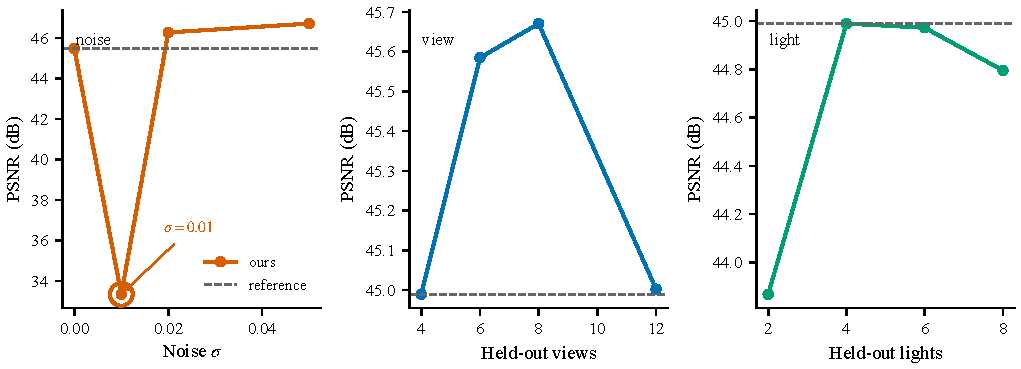
\includegraphics[width=0.95\linewidth]{figures/main/fig6_robustness.pdf}
  \caption{Robustness sweeps for the spot/PartUV accepted case. Light and view sweeps remain stable, while the noise sweep keeps the non-monotonic sigma=0.01 rollback anomaly rather than smoothing it away.}
  \label{fig:robustness}
\end{figure}

\Cref{tab:robustness,fig:robustness} summarize robustness on the spot/PartUV accepted case. Increasing held-out lights from four to eight changes PSNR by at most 0.19 dB, and the two-light setting remains within 1.12 dB. Increasing held-out views from four to 12 is also stable. The noise sweep is less clean: \(\sigma=0.01\) triggers rollback and drops to 33.35 dB, while \(\sigma=0.02\) and \(\sigma=0.05\) accept and recover high PSNR. We retain this non-monotonic anomaly because smoothing it away would overstate stability.

\paragraph*{Bunny robustness sweep.}
\begin{table}[t]
\centering
\scriptsize
\caption{Extended robustness sweeps for spot and bunny (PartUV + ours). Light and view perturbations remain stable; the noise sweep is non-monotonic on both assets and is rejected by C5 at extreme $\sigma$, so the deployed atlas falls back to the baseline.}
\label{tab:robust_extended}
\begin{tabular}{@{}llrrrr@{}}
\toprule
Asset & Sweep & Level & PSNR & Drop & C5 \\
\midrule
spot & light & 2 & 43.87 & +1.12 & accept \\
spot & light & 4 (ref) & 44.99 & 0.00 & accept \\
spot & light & 8 & 44.80 & +0.19 & accept \\
spot & view & 4 (ref) & 44.99 & 0.00 & accept \\
spot & view & 12 & 45.00 & -0.01 & accept \\
spot & noise & 0.01 & 33.35 & +12.13 & rollback \\
spot & noise & 0.05 & 46.71 & -1.23 & accept \\
\midrule
bunny & light & 2 & 39.46 & -0.92 & accept \\
bunny & light & 4 (ref) & 38.53 & 0.00 & accept \\
bunny & light & 8 & 38.24 & +0.29 & accept \\
bunny & view & 4 (ref) & 38.53 & 0.00 & accept \\
bunny & view & 12 & 39.72 & -1.19 & accept \\
bunny & noise & 0.01 & 42.22 & -3.15 & rollback \\
bunny & noise & 0.05 & 24.59 & +14.48 & rollback \\
\bottomrule
\end{tabular}
\end{table}

\Cref{tab:robust_extended} extends the same protocol to the bunny/PartUV accepted case. Light and view sweeps remain stable on bunny too (light drop $\leq$ 0.92 dB, view drop $\leq$ 1.19 dB). The noise sweep on bunny shows the same non-monotonicity as spot, but with a different failure point: at $\sigma$=0.05 PSNR drops 14.48 dB and C5 rolls back, while $\sigma$=0.01 and $\sigma$=0.02 produce candidate PSNR \emph{above} the reference. This rules out a spot-specific artifact: noise-induced PartUV chart restructuring is a generic failure mode of the input atlas family, and our gate correctly rejects it on both assets when held-out evidence does not support deployment.

\section{Confounds, honest disclosure, and analysis}
\label{sec:confounds}

The experiments support a selective deployment method, not a broad UV optimizer. This section makes the confounds explicit: what the accepted gains do not depend on, what they do depend on, and where the current evidence is weak.

\subsection{Strict matched controls}
\label{sec:matched_controls}

\begin{table}[t]
\centering
\scriptsize
\caption{Strict matched-control results. (a) The gain survives atlas-size, padding, and chart-count locks, but disappears under distortion, utilization, or all-lock protocols. (b) Absolute UV-proxy changes for the accepted cases: Q$_{95}$ distortion stays within $\pm$25\% but texture utilization drops 35--60\%; chart count and seam length are unchanged. This quantifies the localized UV-proxy cost the C5 gate is willing to pay for the +10--15 dB PBR gain.}
\label{tab:matched}
\begin{tabular}{@{}lrrll@{}}
\toprule
\multicolumn{5}{@{}l}{\textbf{(a) Relit PSNR delta under matched controls}}\\
Condition & Spot $\Delta$ & Bunny $\Delta$ & matched OK & C5 \\
\midrule
Atlas-size and padding locked & \textbf{+14.67} & \textbf{+10.23} & yes & accept \\
Chart count locked within +/-5\% & \textbf{+14.67} & \textbf{+10.23} & yes & accept \\
Distortion Q95 locked & +0.00 & +0.00 & yes & rollback \\
Texture utilization locked & +0.00 & +0.00 & yes & rollback \\
All strict matched controls & +0.00 & +0.00 & yes & rollback \\
\bottomrule
\end{tabular}

\vspace{0.4em}
\begin{tabular}{@{}lrrrr@{}}
\toprule
\multicolumn{5}{@{}l}{\textbf{(b) Absolute UV-proxy stats for accepted cases (init $\rightarrow$ deployed)}}\\
Asset & $Q_{95}$ distortion & Utilization & Charts & Seam length \\
\midrule
spot/PartUV & 63.80 $\rightarrow$ 62.90 & 0.382 $\rightarrow$ 0.236 & 19 $\rightarrow$ 19 & 22.20 $\rightarrow$ 22.20 \\
bunny/PartUV & 11.02 $\rightarrow$ 13.56 & 0.634 $\rightarrow$ 0.263 & 2 $\rightarrow$ 2 & 11.06 $\rightarrow$ 11.06 \\
\bottomrule
\end{tabular}
\end{table}


\begin{figure}[t]
  \centering
  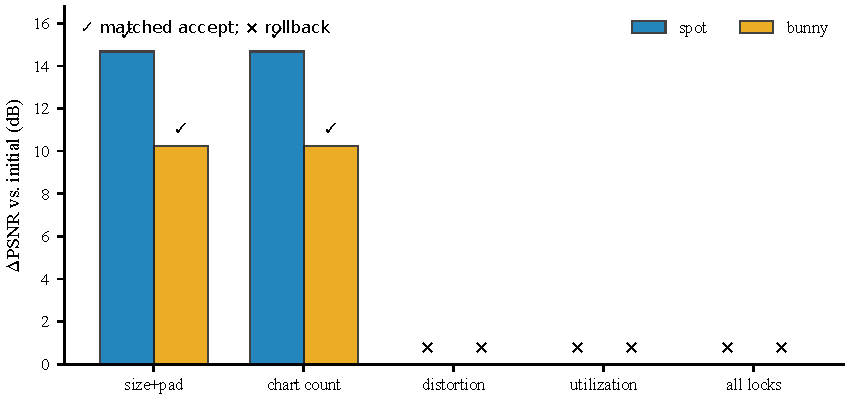
\includegraphics[width=0.95\linewidth]{figures/main/fig5_matched.pdf}
  \caption{Strict matched controls for the accepted PartUV cases. Gains persist when atlas size, padding, or chart count are locked, but vanish under distortion, utilization, or all strict matched controls, indicating a principled downstream-fidelity trade-off.}
  \label{fig:matched_control}
\end{figure}

\Cref{tab:matched,fig:matched_control} rule out three simple explanations. The spot and bunny gains persist when atlas size and padding are locked, and they also persist when chart count is locked within the matched protocol. The method is therefore not merely buying a larger texture, adding padding, or increasing chart count.

The same table also shows the cost of the method. When distortion \(Q_{95}\), packing utilization, or all strict controls are locked, both accepted PartUV cases roll back to baseline. The gain requires localized freedom in distortion and utilization. We interpret this as a principled trade-off: classical UV metrics are useful proxies for atlas geometry and packing efficiency, but they are not equivalent to downstream PBR relighting fidelity. The method spends distortion/utilization slack only when the residual evidence and C5 gate justify the exchange.

\paragraph*{Semantic preservation.}
\begin{table}[t]
\centering
\caption{Chart-part purity comparison (\cref{sec:confounds}). PartUV and our repaired output preserve part semantics perfectly relative to the PartUV part hierarchy; xatlas re-charting reduces purity, with entropy growing on assets that have many small parts.}
\label{tab:purity}
\begin{tabular}{@{}lrrrr@{}}
\toprule
Asset & xatlas Purity & PartUV Purity & Ours Purity & xatlas Entropy \\
\midrule
spot & 0.878 & \textbf{1.000} & \textbf{1.000} & 0.079 \\
bunny & 0.866 & \textbf{1.000} & \textbf{1.000} & 0.509 \\
objaverse & 0.783 & \textbf{1.000} & \textbf{1.000} & 0.594 \\
\bottomrule
\end{tabular}
\end{table}

Chart--part purity gives a quantitative reason not to replace PartUV with xatlas when part organization is a pipeline constraint. Using the PartUV leaf-chart partition as the reference part proxy, xatlas purity is lower on spot, bunny, and the Objaverse asset, while PartUV and our repaired output remain at the reference purity. \emph{This metric is partition-dependent}: by construction, our repair never globally re-charts, and PartUV is taken as the reference partition, so the purity comparison is a direct check of whether xatlas's global re-charting violates the chosen partition. It is therefore a witness for "does PartUV-style chart organization survive repair?" rather than a venue-independent editability score; we treat human-labeled part purity, downstream rig-aware editing, and accessory transfer benchmarks as future evaluation work.

To avoid relying only on the PartUV-derived reference partition, we add the curvature-alignment metric in \cref{tab:curvature_alignment}. It treats high-dihedral mesh edges as a geometry-only proxy for part-like boundaries and computes chart-boundary IoU/precision against that set. This metric still is not a human editing benchmark, but it removes the tautology that PartUV-defined parts automatically favor PartUV-preserving repairs.

\subsection{Selective trigger rate}
\label{sec:selective_trigger}

Across the 12 Main Anchor Evaluation cases and eight Transfer and Robustness Study transfer cases, C5 accepts three repairs and rolls back 17 candidates. The accepted cases are spot/PartUV, bunny/PartUV, and procedural warped cylinder, giving a 3/20 trigger rate over the displayed tested rows. The A1 key-case rerun in \cref{tab:a1_split} separately checks two accepted PartUV cases (spot, bunny) and two rollback controls (spot/xatlas, Objaverse/xatlas) across three disjoint proposal/gate/test split seeds. Accepted PartUV gains persist on the held-out test split (spot $+12.58 \pm 0.83$ dB, bunny $+11.84 \pm 0.89$ dB), and the rollback controls stay at $\Delta = 0.00 \pm 0.00$ dB across all three seeds, so the headline gain is not an artifact of evaluating on the same residual signal that drove repair selection. This is a leakage-control audit rather than a replacement for the full single-seed table. The discrepancy between candidates and deployed outputs is deliberate: the method is allowed to search, but deployment is gated. This matters most for already-good xatlas rows and for procedural transfer rows where a high-PSNR candidate can still violate seam, distortion, or utilization guards. Those candidates are not deployed.

\begin{figure}[t]
  \centering
  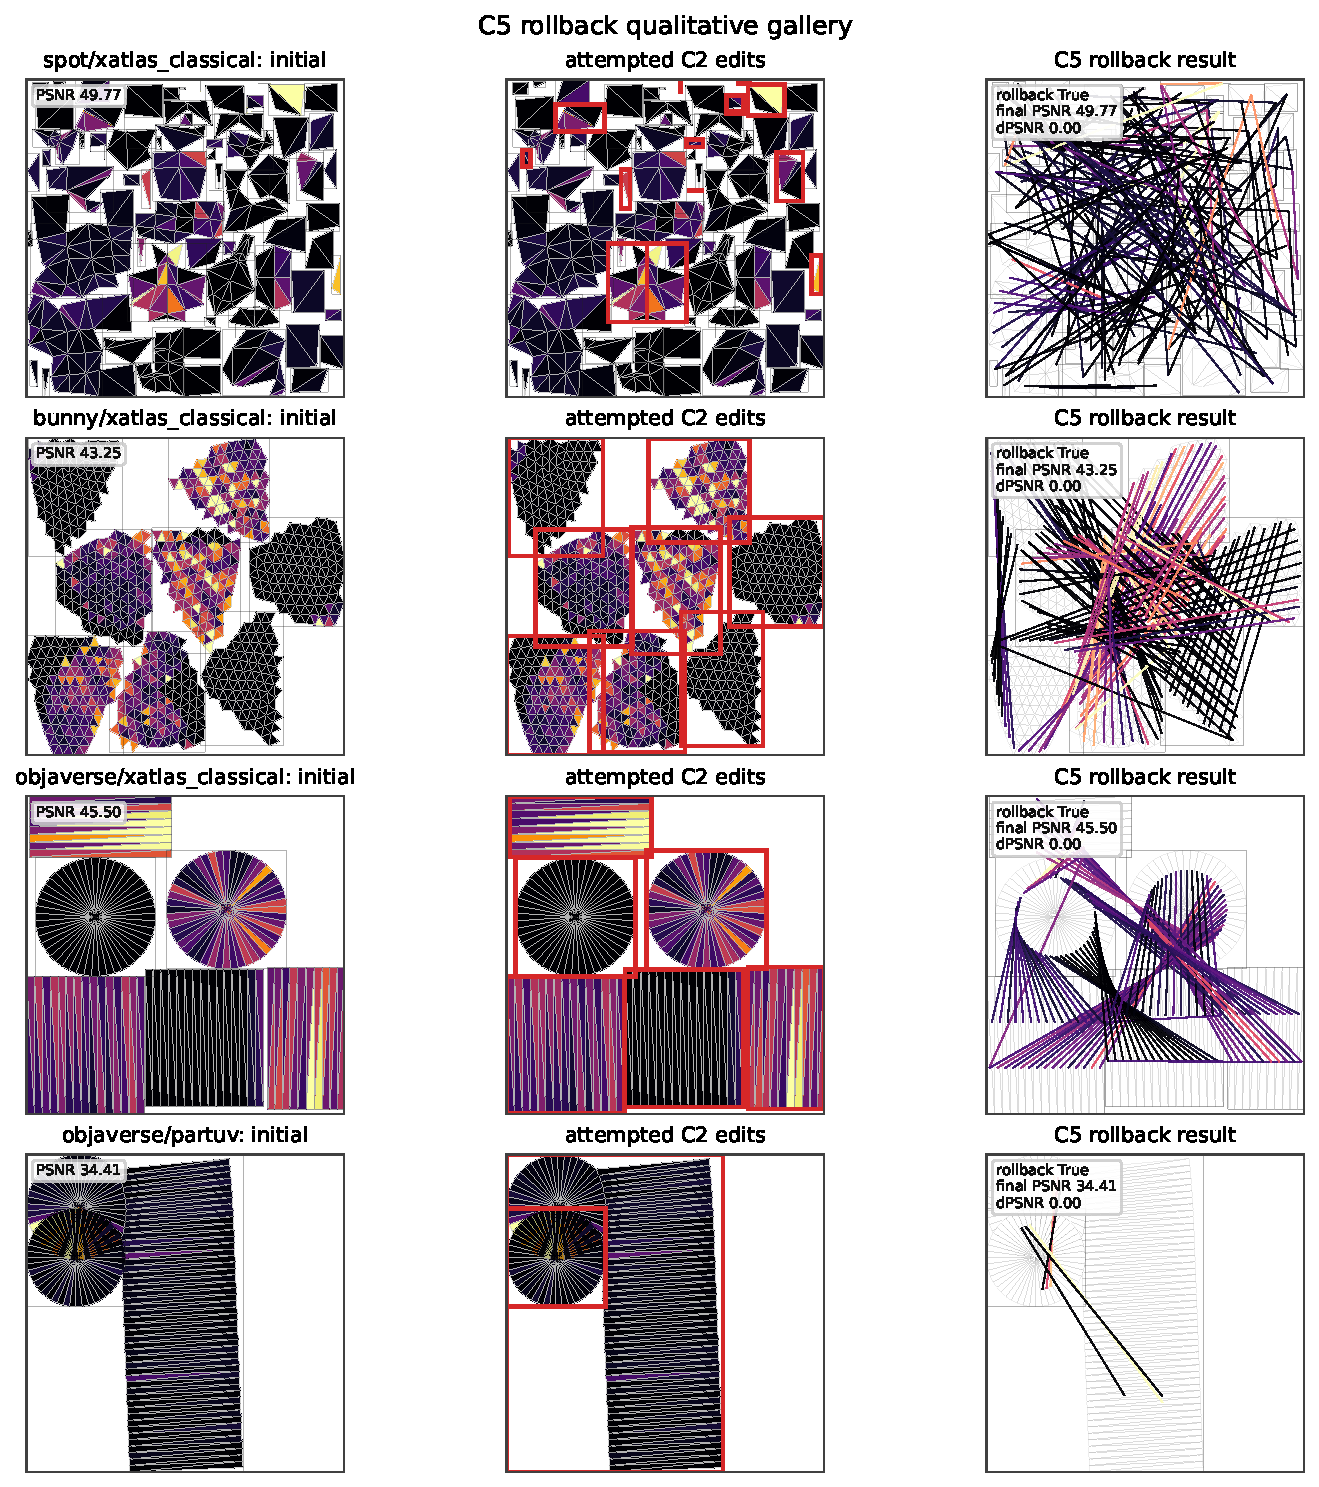
\includegraphics[width=0.95\linewidth]{figures/qualitative_residual_chain/rollback_gallery.pdf}
  \caption{Rollback gallery. The method can propose edits for cases where the residual atlas suggests a possible repair, but C5 deploys the baseline when held-out relighting and seam metrics do not justify the change.}
  \label{fig:rollback_gallery}
\end{figure}

\Cref{fig:rollback_gallery} visualizes this non-harm behavior. It is not evidence that every attempted edit is visually useful; it is evidence that failed candidates can be filtered out before deployment.

\subsection{C4 and weak isolated signals}
\label{sec:c4_disclosure}

C4 is included because PBR seams are cross-channel: albedo, normal, roughness, and metallic discontinuities are not perceptually interchangeable. However, the present ablations do not prove C4 as a standalone necessary component. A5 and A9 are zero-signal in the completed table, and the current hooks may not isolate channel coupling cleanly. We therefore keep C4 as a diagnostic regularizer and reporting tool rather than a top-level claim. The stronger channel evidence comes from A2, where collapsing the baker to RGB-only loses about 12.5 dB.

\subsection{Baseline reproduction scope}
\label{sec:baseline_scope}

The baseline story is intentionally bounded. The main table uses xatlas, Blender Smart UV, real PartUV, and a matched oracle. FlexPara was blocked by Python/PyTorch/CUDA-op/checkpoint constraints, OT-UVGS was treated as an unverified adjacent capacity idea rather than a direct mesh-UV reproduction, and Flatten Anything and ParaPoint were not fully runnable in the available environment. These failures are not hidden; \cref{app:baseline_failure} gives the reproduction table used to scope the claims.

\subsection{Noise anomaly}
\label{sec:noise_anomaly}

The robustness sweep contains a non-monotonic mesh-noise anomaly. At \(\sigma=0.01\), the spot/PartUV case rolls back and PSNR stays at the baseline 33.35 dB; at \(\sigma=0.02\) and \(\sigma=0.05\), the method accepts and recovers high PSNR (46.28 and 46.71 dB). The PartUV chart count grows monotonically with noise (19, 22, 23, 25 charts for \(\sigma\in\{0,0.01,0.02,0.05\}\)) and the baseline \(Q_{95}\) distortion is in the same range (59--64) across all four cells, so the anomaly is not driven by a structural break in the upstream atlas family. The mechanism is more local: at \(\sigma=0.01\), the C2 candidate's chart count and \(Q_{95}\) distortion are bit-identical to the baseline (22 charts, \(Q_{95}=59.03\)), meaning the residual signal was not concentrated enough to motivate any chart-level action and the candidate is just the baseline atlas reproduced; C5 then correctly rolls back. At \(\sigma=0.02\) and \(\sigma=0.05\) the residual structure exceeds the C2 selection threshold (\cref{eq:topk}), the candidate moves \(Q_{95}\) by +2.0 and +0.8 respectively under the same chart count, and C5 accepts. The anomaly is therefore consistent with a small-noise dead zone in the C2 selection rule rather than a C5 gate fluke or a method failure under deployment; \cref{tab:robustness} retains the row so this dead zone is visible to the reader. Closing this gap would require lowering the C2 top-K threshold for noise-perturbed meshes, which is intentionally not done in this submission because the protocol fixes all C2/C3/C5 thresholds a priori (\cref{sec:implementation}).

\section{Limitations and future work}
\label{sec:limitations}

The method is limited to a single UV atlas shared by all PBR channels. This matches the target DCC workflow, but it excludes multi-atlas, UDIM-heavy, or per-channel UV strategies that could improve appearance while changing production constraints. The method also assumes that disjoint proposal, gate, and test relighting sets are available or can be approximated; when the material source is itself unreliable, residual attribution may mix atlas error with material-prediction error.

The generated-asset evaluation remains limited. The eight headline transfer meshes are procedural noisy shapes, and the real-mesh evidence covers five SDS-pipeline init shapes from two independent repositories (Fantasia3D \cite{chen2023fantasia3d} and threestudio \cite{guo2023threestudio}); two accept (\texttt{f3d\_animal}, \texttt{ts\_animal}) and three roll back. This is enough to show the same C1--C5 mechanism transfers to independently generated meshes, but it is not a statistical claim about Trellis-3D \cite{xiang2024_trellis_structured_3d_latents}, GET3D \cite{gao2022_get3d_generative_model}, DreamFusion-style \cite{poole2023_dreamfusion_text_to_3d}, or broader production generated outputs. A larger real generated-mesh sweep, including the Objaverse curated subset and Polyhaven that timed out under our per-mesh PartUV preprocessing budget, remains future work.

Several components need cleaner isolation. C4 seam coupling has engineering value as a diagnostic, but its current A5/A9 ablations show zero isolated signal. The explicit mip term in C3 is also weak in the current table, even though residual-aware allocation helps. Future experiments should use seam-specific stress assets, verified ablation hooks, and controlled mip-frequency cases rather than relying on the main spot/bunny assets alone.

Robustness is also bounded. The light, view, and noise sweeps are demonstrated for both spot and bunny PartUV (\cref{tab:robustness,tab:robust_extended}), while the new leakage-control rerun is intentionally limited to key accept/rollback cases with multiple split seeds. Extending both robustness and multi-seed leakage checks to the full 12-case table, warped cylinder, and additional generated meshes is left for future work, and the noise anomaly at extreme $\sigma$ is intentionally retained rather than smoothed away.

The matched-control results also limit the claim. The method's gain disappears when distortion tail and utilization are fully locked. This is not a hidden bug, but it means the method is unsuitable for pipelines that require strict preservation of those classical UV metrics. Finally, dynamic or 4D assets are not evaluated. Temporal stability of the residual atlas, chart edits, and texel allocation remains open.

\section{Conclusion}
\label{sec:conclusion}

This paper argues that PBR baking residual should be treated as a first-class atlas quality signal for selective UV atlas repair. Geometry-based UV metrics remain necessary, but they can miss the failures users see after baking and relighting: residual hot spots, mip leakage, and cross-channel seam artifacts. The proposed differentiable baking-error atlas localizes those failures, proposes only local repairs to a fixed upstream atlas, reallocates a fixed texel budget, and deploys the result only through a matched-control gate.

The evidence supports a selective method. In the accepted spot/PartUV, bunny/PartUV, and warped-cylinder cases, relit \PSNR{} improves by roughly 10--15 dB. In the other tested cases, C5 rolls back and preserves the baseline. The matched-control study makes the trade-off explicit: the gain is not from atlas size, padding, or chart count, but it does require localized distortion and utilization freedom. That is the practical message of the draft. Residual-driven repair can improve PBR fidelity when atlas proxies fail, but it should be deployed as a gate, not as an unconditional replacement for production UV tools.


\appendix
\section{Implementation details}
\label{app:implementation}

\paragraph*{C2 local actions.}
For each selected chart, split proposes a cut along the dominant curvature direction estimated from per-face normals and the chart covariance frame. Merge-with-neighbor evaluates adjacent charts in nearest-neighbor order by seam residual and keeps the merge with the lowest C2 score. Boundary slide moves boundary texels for \(N\) small steps along the gradient flow of the face residual \(e_f\), clamped by the distortion guard. Local ARAP keeps the chart center anchored and runs 10 local/global iterations before repacking the chart under the fixed atlas-size budget.

\paragraph*{Beam scoring and residual attribution.}
Candidates are scored in the order split, merge, boundary slide, and local ARAP for each selected chart, then pruned to beam size 4. The render term in \cref{eq:c2_cost} is measured as
\begin{equation}
\Delta\mathcal{L}_{render}(c,a)=
\mathcal{L}_{render}(U_{c,a})-\mathcal{L}_{render}(U_0),
\end{equation}
on the proposal split $\Vprop \times \Lprop$ only; this split is disjoint from the gate split $\Vgate \times \Lgate$ used by C5 and from the test split $\Vtest \times \Ltest$ used to report headline metrics (\cref{sec:exp_setup,tab:a1_split}). Residual attribution uses the nvdiffrast face-id buffer: per-pixel proposal-split RGB residuals are scattered with \(\mathrm{scatter\_add}\) into a per-face accumulator and normalized by the visible sample count before chart aggregation.

\paragraph*{Runtime and memory.}
\begin{table}[t]
\centering
\scriptsize
\caption{End-to-end wall-clock and peak GPU memory for representative cases on a single RTX 4090 (PyTorch 2.7.1 cu128, bf16 baker). Wall-clock includes oracle PBR setup, baking, residual attribution, candidate search, C5 audit, and final atlas export; PartUV preprocessing of the upstream atlas is excluded and reported separately.}
\label{tab:runtime}
\begin{tabular}{@{}lrrrl@{}}
\toprule
Case & Faces & Wall-clock (s) & Peak GPU (GB) & C5 \\
\midrule
spot / PartUV (accept) & 372 & 1313 & 0.59 & accept \\
bunny / PartUV (accept) & 1280 & 1814 & 0.59 & accept \\
spot / xatlas (rollback) & 372 & 2578 & 0.53 & rollback \\
objaverse / xatlas (rollback) & 192 & 166 & 0.53 & rollback \\
proc\_warped\_cylinder / PartUV (accept) & 1152 & 158 & 0.58 & accept \\
ts\_animal / PartUV (real, accept) & 3068 & 2777 & 0.59 & accept \\
f3d\_animal / PartUV (real, accept) & 3068 & 16772 & 0.96 & accept \\
\bottomrule
\end{tabular}
\end{table}

\Cref{tab:runtime} reports end-to-end wall-clock and peak GPU memory on a single RTX 4090. Procedural and small-asset cases finish in 2--5 minutes; larger meshes (bunny, ts\_animal, f3d\_animal) need 30~min--5~h dominated by C2 candidate search rather than rendering. Peak GPU memory stays under 1~GB for all listed cases. PartUV upstream preprocessing is independent and is the practical bottleneck for the 18 deferred real meshes (\cref{sec:limitations}); the differentiable baker, residual attribution, C2 search, and C5 audit themselves do not require multi-GPU.

\paragraph*{Renderer and C5 thresholds.}
The renderer uses nvdiffrast \(\mathrm{rasterize\_cuda}\) for visibility, a custom GGX shader for albedo/normal/roughness/metallic relighting, fp16 texture and shading buffers, and fp32 reductions for metrics. The logged C5 gate uses \(\delta_p=0.3\) dB, \(\delta_s=8\%\) relative seam drop, \(\epsilon_D=3.0\) for maximum distortion \(Q_{95}\), and \(\Delta_C=\pm10\%\) chart-count tolerance.

\section{Baseline reproduction failure table}
\label{app:baseline_failure}

\begin{table*}[t]
\centering
\scriptsize
\caption{Baseline reproduction scope. Only real integrated baselines are used for main numerical comparisons; partial or failed baselines are reported to bound the claims.}
\label{tab:baseline_failure}
\begin{tabularx}{\linewidth}{@{}l l l X@{}}
\toprule
Baseline & Status & Used in main table & Reproduction note \\
\midrule
xatlas & real & yes & Python xatlas integration ran on all three main assets and passed the matched protocol. \\
Blender Smart UV & real & yes & Blender 3.0.1 Smart UV ran after wrapper fixes; it is a useful production baseline but often violates chart-count or utilization matching because it follows a different atlas paradigm. \\
PartUV & real & yes & Real subprocess integration produced part-aware atlases for spot, bunny, and Objaverse; PartUV is the primary weak-baseline case where residual repair triggers. \\
matched oracle & real control & yes & Self-implemented oracle UV reference used as an upper-bound control; infinite PSNR rows are rolled back because there is no residual-backed improvement to deploy. \\
FlexPara & partial & no & Repository constraints required Python 3.9, PyTorch 1.10/CUDA 11.1 compatibility, custom CUDA ops, and unavailable shipped checkpoints; only a proxy was available, so it is excluded from main claims. \\
OT-UVGS & adjacent/proxy & no & Treated as a capacity-allocation reference rather than a verified mesh-UV baseline; no full direct mesh reproduction is claimed. \\
Flatten Anything & failed & no & Environment and checkpoint requirements could not be verified in the available run budget. \\
ParaPoint & failed & no & Repository or checkpoint availability was not verified, so no numerical comparison is claimed. \\
visibility-param control & proxy & no & Included as an explicit attempt at the review guardrail baseline, but no public implementation was available for a real reproduction. \\
\bottomrule
\end{tabularx}
\end{table*}

\section{Additional qualitative result}
\label{app:additional_qual}

\begin{figure*}[t]
  \centering
  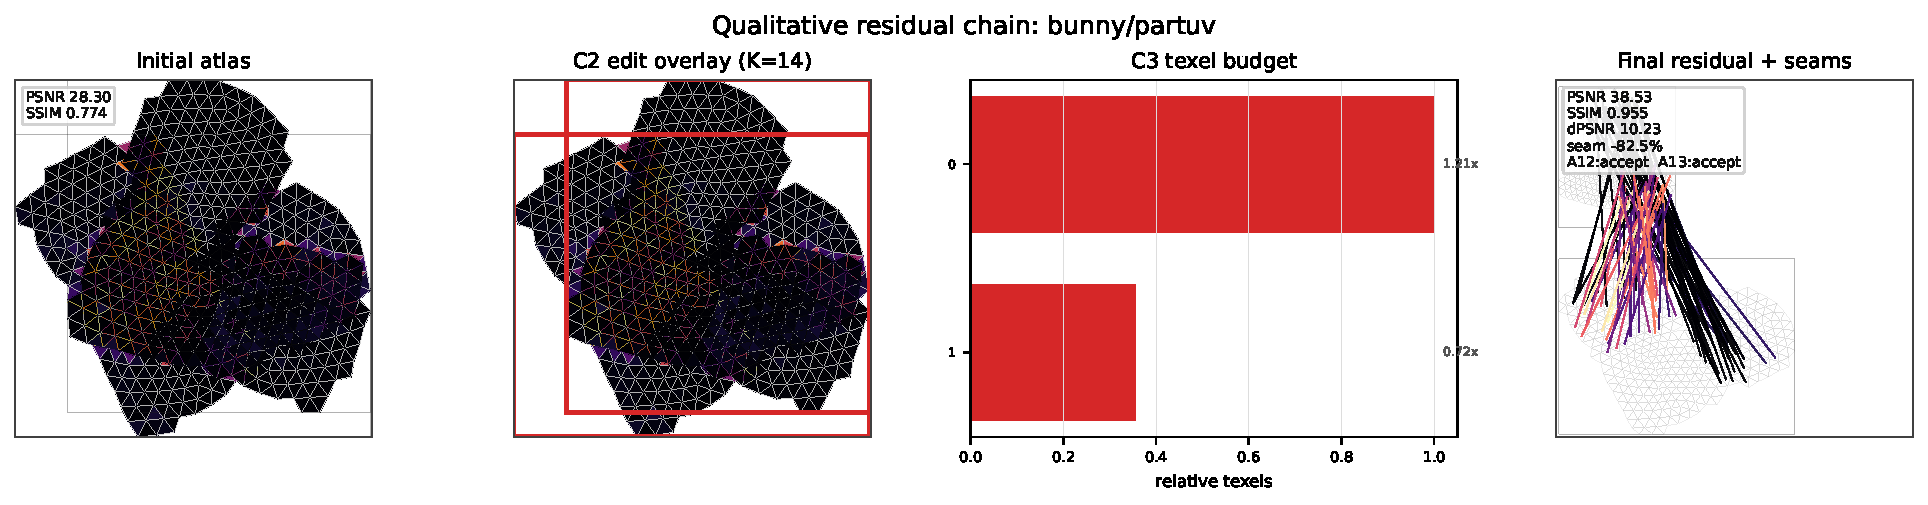
\includegraphics[width=0.88\linewidth]{figures/qualitative_residual_chain/bunny_partuv_residual_chain.pdf}
  \caption{Bunny/PartUV residual chain. The same residual-driven pipeline accepts the local repair and improves relit \PSNR{} from 28.30 dB to 38.53 dB.}
  \label{fig:bunny_chain}
\end{figure*}

\Cref{fig:bunny_chain} complements the spot hero case in \cref{fig:spot_chain}. The bunny atlas has fewer charts, so the edited-chart ratio is high even though the absolute edit count is small. This is why the paper reports edited counts and not only edited percentages.


\bibliographystyle{egPublStyle-PG2026/eg-alpha}
\bibliography{references}

\end{document}
